\documentclass[11pt, a4paper, oneside]{Thesis}
\usepackage{etex}
\usepackage{array}
\usepackage{float}
\usepackage{subcaption}
\usepackage{amsmath}
\usepackage{tocbibind}
\usepackage{multirow}
\usepackage{setspace}
\usepackage{tikz}
\usetikzlibrary{shapes.geometric, arrows}
\usepackage{microtype}
\usepackage{standalone}
\usepackage{tabularx}
\usepackage{booktabs}
\usepackage[normalem]{ulem}
\useunder{\uline}{\ul}{}
\usepackage{graphicx}
\usepackage{titlesec}
\graphicspath{ {figures/} }
\usepackage[toc,page]{appendix}
\usepackage[ruled,vlined,linesnumbered]{algorithm2e}
\usepackage[utf8]{inputenc}
\usepackage[acronym, toc]{glossaries}
\usepackage{pdfpages}
\usepackage{datetime}
\usepackage{pdfpages}

\newdate{date1}{28}{03}{2018}
\newdate{date2}{29}{03}{2018}

\date{\displaydate{date1}}

\date{\displaydate{date2}}
\makeglossaries

\newcolumntype{Y}{>{\centering\arraybackslash}X}
\newcolumntype{L}{>{\centering\arraybackslash}m{3cm}}
\setlength{\parindent}{0.7cm}

\makeatletter
\DeclareRobustCommand\onedot{\futurelet\@let@token\@onedot}
\def\@onedot{\ifx\@let@token.\else.\null\fi\xspace}

\titleformat{\paragraph}
{\normalfont\normalsize\bfseries}{\theparagraph}{1em}{}
\titlespacing*{\paragraph}
{0pt}{3.25ex plus 1ex minus .2ex}{1.5ex plus .2ex}

\def\eg{\emph{e.g}\onedot} \def\Eg{\emph{E.g}\onedot}
\def\ie{\emph{i.e}\onedot} \def\Ie{\emph{I.e}\onedot}
\def\cf{\emph{c.f}\onedot} \def\Cf{\emph{C.f}\onedot}
\def\etc{\emph{etc}\onedot} \def\vs{\emph{vs}\onedot}
\def\wrt{w.r.t\onedot} \def\dof{d.o.f\onedot}
\def\etal{\emph{et al}\onedot}
\usepackage[group-separator={,}]{siunitx}

\makeatother

\newcommand{\argmax}{\operatornamewithlimits{argmax}}
\newcommand{\argmin}{\operatornamewithlimits{argmin}}
\newcommand{\abs}[1]{\left\lvert#1\right\rvert}
\newcommand{\norm}[1]{\left\lVert#1\right\rVert}
\newcommand{\listofalgorithmes}{\tocfile{\listalgorithmcfname}{loa}}
\newcommand\Chapter[2]{
  \chapter[#1: {\itshape#2}]{#1\\[1ex]\Large#2}
}

	\begin{document}
\input{commands}
\newacronym{wu}{WU}{Warm Up}
\newacronym{fmarc}{F-MARC}{FIFA Medical and Research Centre}
\newacronym{avg}{AVG}{Active Video Gaming}
\newacronym{sdt}{SDT}{Self Determination Theory}
\newacronym{cet}{CET}{Cognitive Evaluation Theory}
\newacronym{oit}{OIT}{Organismic Integration Theory}

%\setcode{utf8}

% *************** Front matter ***************
\frontmatter

\title  {ImMotion\\ An Exergame for Warm Up Guidance}

\authors  {\texorpdfstring
            {{Marko Vuji\'c}}
            {}
            }
\addresses  {\groupname\\\deptname\\\univname}  % Do not change this here, instead these must be set in the "Thesis.cls" file, please look through it instead
%\usdate
\date       {Saarbr\"ucken, \today }
\subject    {}
\keywords   {}

\maketitle

%\newpage
%\mbox{}
%\thispagestyle{empty}
%\newpage

\setstretch{1.3}

\thispagestyle{empty}
\setcounter{tocdepth}{5}
\section*{Eidesstattliche Erkl\"{a}rung}
Ich erkl\"{a}re hiermit an Eides Statt, dass ich die vorliegende Arbeit selbstst\"{a}ndig verfasst und keine
anderen als die angegebenen Quellen und Hilfsmittel verwendet habe.

\vspace{0.60cm}
\section*{Statement in Lieu of an Oath}
I hereby confirm that I have written this thesis on my own and that I have not used any other media or
materials than the ones referred to in this thesis.
\vspace{1.5cm}

\section*{Einverst\"{a}ndniserkl\"{a}rung}
Ich bin damit einverstanden, dass meine (bestandene) Arbeit in beiden Versionen in die Bibliothek der
Informatik aufgenommen und damit ver\"{o}ffentlicht wird.

\vspace{0.60cm}
\section*{Declaration of Consent}
I agree to make both versions of my thesis (with a passing grade) accessible to the public by having
them added to the library of the Computer Science Department.
\vspace{3cm}

\begin{flushright}
\noindent Saarbr\"{u}cken, \today
\hfill
Marko Vuji\'c
\end{flushright}

\clearpage  % Declaration ended, now start a new page
%% ----------------------------------------------------------------

%%\newpage
%\mbox{}
%\thispagestyle{empty}
%\newpage

% The Abstract Page
\addtotoc{Abstract}  % Add the "Abstract" page entry to the Contents
\abstract{Past research related to exergames has found that they can help to motivate people to exercise by converting physical activity into an enjoyable game. However, these exergames have been single purpose usually home fitness only. In this thesis, we designed an exergame for warm up guidance to be used in gyms and fitness centers before physically more strenuous exercise. We utilized immersive technologies based on the hypothesis that they can be used as a guiding tool for warm up procedures, would increase warm up duration, and increase exercise enjoyment.  In order to evaluate our exergame we have conducted two user studies. The first was an online study where we collected responses from 466 participants about their work out and warm up habits. For the second study we utilized a between-subject laboratory experiment with two conditions: (a) warming up by following a video with a fitness instructor performing a warm up session; (b) warming up by interacting with our exergame solution. The results showed a statistically significant increase of exercise duration, enjoyment of the physical activity, and participant's momentary feeling of pleasure relative to the non-gaming condition. 
%Based on our findings from both the studies, we concluded that by making the exergame interactive and appealing it is possible to transform the warm up procedure from a repetitive and tiresome activity to an entertaining and challenging necessity.% The exergame showed a significant increase in user motivation and enjoyment when compared to the non gaming condition, with the Kinect condition found to be slightly more motivating than the screen condition.
\addtocontents{toc}{\vspace{1em}}  % Add a gap in the Contents, for aesthetics
\clearpage
%% ----------------------------------------------------------------
%\newpage
%\mbox{}
%\thispagestyle{empty}
%\newpage

\setstretch{1.3}  % Reset the line-spacing to 1.3 for body text (if it has changed)

% The Acknowledgements page, for thanking everyone
\acknowledgements{
\addtocontents{toc}{}  % Add a gap in the Contents, for aesthetics    \vspace{1em}


}
\clearpage  % End of the Acknowledgements
%% ----------------------------------------------------------------
%\newpage
%\mbox{}
%\thispagestyle{empty}
%\newpage

%\newpage
%%\mbox{}
%\thispagestyle{empty}
%\newpage

\setstretch{1}
\begin{spacing}{0.1}
\pagestyle{fancy}
\tableofcontents
%\newpage
\listoffigures	
%\newpage
%\listoftables
%\newpage
%\listofalgorithmes
\end{spacing}

\clearpage

\setstretch{1.3}
% *************** Main matter ***************
\mainmatter
%\printglossary[type=\acronymtype]
%\chapter{Introduction}
\label{chap:intro}

\section{Motivation}
\label{chap:motivation}

%\chapter{Literature review}\label{chapter:warmup}

The following chapter provides an overview of the past research related to the warm-up as a preparatory exercise prior performing physical activity and conceptually related works in the domain of gamified solutions relevant to fitness and exercise. To impose structure, first the basic concepts related to warm-up and an overview of studies and results regarding the benefits of warm-up is given. Following, the concept of gamification is introduced and most relevant ... in ... At the end of this chapter, a comparison between the presented approaches and our solution is made.
\section{Warm up in sports}
\subsection{Introduction}
Despite very contrasting believes and limited scientific evidence regarding it's effectiveness in many situations, warm-up (WU) has become a standard practice among professional and
recreational athletes \cite{bishop2003warm1, bishop2003warm2, shellock1985warming}. WU in sports is defined as a period of preparatory exercise which is carried out in order to prepare the athlete for the demands of the subsequent physical activity \cite{karvonen1992importance, woods2007warm, hedrick1992exercise}.
%karvonen skini i procitaj
Typically, WU includes a short and low-intensity preparatory activity which is followed by a stretching routine and sport specific exercise \cite{safran1989warm}. 
The purpose of WU is to enhance the subsequent competition or training performance and improve muscle dynamics to reduce the risk of sport-related injury\cite{bishop2003warm1, shellock1985warming, knudson2008warm}. 
 %HERE MENTION THE STUDIES THAT SAY THIS DOESNT HELP.  CHECK LEMON ILIEV
Nonetheless, there is still deficiency of scientific evidence on what kind of WU can influence both muscle damage prevention and performance improvement \cite{safran1989warm}.\\ %cite
\subsection{WU benefits}
Fradkin \textit{et al.} carried out a systematic review and meta-analysis of relevant studies concerning the benefits of WU on the performance. They found that an adequate WU supports an improvement in performance in 79\% of the research studies analyzed. Furthermore, they pointed out that there exist little evidence supporting detrimental effects WU might have on performance and sports participants.
WU can affect the performance via variety of temperature and non-temperature related mechanisms \cite{bishop2003warm1}. 
%By performing a low intensity training routine before taking part in more demanding exercise, an increase in one's body temperature \(Magnusson 
%et al., 2000\) and muscle blood flow occurs \(Tiidus \& Shoemaker, 1995\).  
The most relevant effects of WU can be attributed to physiological mechanisms like increased muscle temperature, decreased resistance of muscle and joints (decreased stiffness), increased oxygen delivery to muscles, increased nerve-conduction rate and speeding of metabolic reactions \cite{bishop2003warm1}. 
However, the benefits of WU are not exclusively physical. Apart from the physiological changes a body undergoes during this preparatory period, it has been hypothesized that a possible psychological benefit can also be gained by following a proper WU routine \cite{bishop2003warm1,shellock1985warming}.
It has been suggested that WU can serve as preparatory phase providing time for athlete to concentrate and mentally prepare for the forthcoming exercise \cite{shellock1985warming}. 
%Thus, possible psychological benefits is increased mental preparedness for the forthcoming exercise\cite{bishop2003warm1}. 
For instance, in the study that investigated the link between a WU and psychological processes, Ladvig (2013) reported that athletes who reported performed a proper WU routine before engaging in more demanding physical activity demonstrated significantly higher levels of exercise related motivation and enjoyment. Thus increased motivation and enjoyment is an additional psychological benefit of WU \cite{ladwig2013psychological}.
 %findings of this theisis: http://aut.researchgateway.ac.nz/bitstream/handle/10292/325/WeerapongP.pdf?sequence=1
\\Apart from physiological and psychological benefits, WU has been suggested to have an important role in sports-related injury prevention \cite{shellock1985warming}. Unfortunatelly, there exist no high-quality research studies in order to draw definite conclusion as to the effect WU has on sports-related injury prevention \cite{fields2007should}. Safran, \textit{et al.} proposed a possible bio-mechanical explanation for injury reduction with WU. The results of this study reported that warmed-up muscles in the animal models can elongate more before failure caused by increased force and length of stretch \cite{safran1989warm}. In the study of Fradkin, \textit{et al.} the current evidence regarding WU in injury prevention has been assessed. Out of five high-quality studies with sufficient data that have been systematically reviewed, three studies reported significant injury related reduction by performing WU before the physical activity while in other two no benefits were reported. Overall, based on the weight of evidence, it has been concluded in favor of WU to decrease the risk of injury.\\
%Furthermore, Nosaka and Clarckson found that high and low intensities of WU could reduce the magnitude musculatory damage ... They proposed that 
%A search of the literature identified only one published research paper on the effects of warm-up on the severity of muscle damage (Nosaka & Clarkson, 1997).  Nosaka and Clarkson (1997) found that both high (100 repetitions of maximal concentric contraction) and low (100 repetitions of minimal concentric contraction) intensities of 
%warm-up could reduce the magnitude of mu
%scle damage as indicated by reduced 
%soreness sensation, strength and range of 
%motion loss, swelling, and creatine kinase 
%activity.  The authors proposed that warm-up 
%might help to increase muscle temperature 
%and circulation, and consequen
%tly, increase muscle and conne
%ctive tissue el
%asticity
%the majority of effects of warm up have been attributed to temperature related mechanism
\subsection{WU types}
There exist various types of WU procedures professional and recreational athletes use as a preparatory phase for the physically more demanding exercise preparation. It is important to distinguish between WU and stretching activities. While WU mainly focuses on core body temperature elevation, stretching involves movements that stretch the muscle in order to increase the range of motions of joints or group of joints \cite{knudson2008warm}. 
Generally, WU procedures can be classified into active and passive WU procedures, and are centered on increase in core and muscle temperature. However, active and passive WU accomplish this objective through different approaches. The former involves raising muscle or core temperature by some external means (e.g. hot showers, saunas), while the latter aims to increase the body temperature through active movements of the major muscle groups (e.g. jogging, cycling, swimming) \cite{shellock1985warming, bishop2003warm2}. The most effective WU that could potentially effect the subsequent performance generally depends on the duration, intensity and the nature of the sports activity to be performed \cite{bishop2003warm2}. As each sport has its own unique requirements, it is difficult to specify a general WU routine that is beneficial and have positive impact by maximizing the subsequent performance. Nonetheless, it is suggested that a proper WU should use general, whole-body movements and last 5-10 minutes which is followed by a 5 minutes recovery period \cite{bishop2003warm2}.  
%dodaj za fatigue
%Several studies were conducted in the 1950s-1970s to investigate the effects of warming-up on athletic performance
%(Richards, 1968). In this context, approximately 60% of these studies found that warm-up was better
%to perform than no warm-up, whereas ~11% found that no warm-up was better, and the remaining ~29% found
%no significant differences between different protocols of warm-up and no warm-up (Blank, 1955). 
%tu sad das ove linkove
%(Generally, a warm-up to minimize impairments and enhance performance should be composed of a submaximal intensity aerobic activity followed by large amplitude dynamic stretching and then completed with sport-specific dynamic activities.
%these say that some stretching is ok
%http://www.jospt.org/doi/pdf/10.2519/jospt.1994.19.1.12
%https://www.ncbi.nlm.nih.gov/pubmed/21373870
%The efficacy, and characteristics, of warm-up and re-warm-up practices in soccer players: a systematic review. This review demonstrated that a static stretching WU reduced acute subsequent performance, while WU activities that include dynamic stretching, PAP-based exercises, and the FIFA 11+ can elicit positive effects in soccer players. The efficacy of an active RWU during half-time is also justified.
%ovo se placa nesto 
 %http://greatist.com/fitness/stretching-dynamic-warmup-040413
\\Although, considering the aforementioned benefits, is widely recommended to undertake the practice of WU, many amateur and recreational athletes do not seem to perform a proper WU before an exercise \cite{fradkin2010effects}. The reasons for this are manifold. Some people do not realize the importance of WU, find it tiresome or pressed for time and eager for instantaneous results, start with the more strenuous activity immediately. A recent survey carried out by Fradkin, \textit{et al.} including 1040 golfers and their WU habits, revealed the most common reasons for not warming-up. The survey showed that out of all the questioned golfers, over 70\% never or rarely warm-up. The most common reasons for not performing a proper WU routine were the perception that WU is needless (38.7\%), lack of time (36.4\%) and that they do not want to be bothered with this routine (33.7\%).
% A survey of 1040 randomly selected golfers was conducted over a 3-week period in July 1999. Information about golf participation, usual warm-up habits and reasons for these warm-up behaviours was obtained by a verbally administered self-report survey. Over 70% of the surveyed golfers stated that they never or seldom warm-up, with only 3.8% reporting warming-up on every occasion. The most common reasons why golfers warmed-up included to play better (74.5%), to prevent injury (27.0%), and because everyone else does (13.2%). Common reasons for not warming-up were the perception that they don't need to (38.7%), don't have enough time (36.4%) and can't be bothered (33.7%).
These results suggest that educational and motivational solutions with primary focus on benefits of WU, including injury prevention, need to be developed and implemented in order to increase the proportion of athletes who engage in WU routines before every strenuous exercise. One possible solution is the usage of \textit{gamification} in motivating athletes to perform WU more regularly. 
\pagebreak
\section{Gamification}
\subsection{Definition}
%http://link.springer.com/chapter/10.1007%2F978-3-319-07127-5_23
%(http://www.enterprise-gamification.com/mediawiki/index.php?title=Category:Gamification_Design_Elements)
% are commonly used 
%check this here https://badgeville.com/wiki/health
%% add gamification example reference
% http://www.enterprise-gamification.com/mediawiki/index.php?title=Gamification_Examples
In recent years, there have been an tremendous increase in popularity of video games inspired software solutions designed to address issues in variety of functional areas, incentivize consumer behavior or increase motivation and desire for achievement. What these software solutions all have in common is that they are based on the concept of \textit{gamification}. This term has begun to rise in popularity in 2010 (Figure \ref{fig:buzz}), and since then has been a trending topic. %ovde dodaj 
%It has proved to be an effective tool for certain businesses for developing new skills, solve problems, improve results or address.
\begin{figure}[h]
    \centering
    \includegraphics[width=\textwidth]{buzz}
    \caption{Google search frequency of the term \textit{gamification} from Janauary 2010 through January 2017. Data source: Google Trends, www.google.com/trends}
    \label{fig:buzz}
\end{figure}
Gamification is being used and studied in various domains, from education and academic performance to health care, finance, company culture building and recruitment, to name a few \cite{gamificationExamples, gamificationWiki, enterpriseGamify}. Large companies like Nike \cite{nikePlus}, Deloitte \cite{deloitte}, Starbucks \cite{starbucks}, Coca Cola \cite{coke} and Toyota \cite{toyota} have all used gamified solutions. %cite the examples and change this sentance. cite https://badgeville.com/wiki/Gamification_Examples
Moreover, there is an increasing number of startups that base their services on the gamification concept \cite{codeacademy} or offer assistance to enterprises to gamify their existing services \cite{badgeville}. Hamari \textit{et al.} reported on an increasing popularity of gamification related researches in the academia \cite{hamari2014does}. Figure \ref{fig:pub} gives an overview of the increase of writing on this topic. The figure includes only the number of publications for every year for the term \textit{gamification} and excludes patents and citations. 
\begin{figure}[h]
    \centering
    \includegraphics[width=\textwidth]{pub}
    \caption{Search hits on 'gamification'. Data source: www.scholar.google.com}
    \label{fig:pub}
\end{figure}
It is worth noticing that the appearance of term gamification publication titles' has been increasing more rapidly than search hits for the same term (see Figure \ref{fig:buzz}). This suggests that gamification is becoming more popular in academic inquiry. 
Detering \textit{et al.} (2011) define gamification as ``the use of game design elements in a non-game context''  \cite{deterding2011game}. In parallel with this term, a verb \textit{to gamify} has been defined. It's meaning reffers to applying game mechanics to supercharge user engagement, loyalty and fun \cite{toGamify}. It should be noted that the definition of gamification outlined by Detering \textit{et al.} relates to \textit{games} and not \textit{play} \cite{deterding2011game}. Even though often used interchangeably, there exists a complex relationship between these two concept and clear distinction can be made. That is, according to the forms they take in the world, \textit{play} can be interpreted as a broader category that includes \textit{game} as a subset \cite{salen2004rules}. Play is normally assumed to be a free-form activity lacking constraints engaged in for pleasure and amusement rather than a serious or practical purpose, whereas games provide context for actions and are limited in action by fixed rules \cite{juul2011half}. In addition, Salen and Zimmerman define game as a system where players engage in an artificial conflict which is defined by rules that limit players behavior and define the game, that can result in a quantifiable outcome or goal \cite{salen2004rules}.
Game design elements represent parts of games used as a building block for creating gamified applications. They are tools and rules that define the overall context of game \cite{gamDesElem}. This means that the definition distinguishes gamification from other systems that employ full-fledged games rather than elements of game design only. Furthermore, it does not include all game elements either, only a subcategory called game design elements. %ova dve poslednje recenice odavde, izmeni 
%http://ludus.hu/en/gamification/
Game design elements are themselves difficult to specify and often are described on varying levels of abstraction. Derived from the available literature, Deterding et al. found that previously identified game elements fell into five distinct levels of abstraction. Table \ref{table:gameElements} lists the five levels of game elements, ordered from concrete to abstract.

\pagebreak
% Please add the following required packages to your document preamble:
% \usepackage[normalem]{ulem}
% \useunder{\uline}{\ul}{}
\begin{table}[]
\centering
\caption{Taxonomy of game design elements by level of abstraction}
\label{table:gameElements}
\begin{tabular}{lll}
\hline
\textbf{Level} & \textbf{Description} & \textbf{Example} \\ \hline
\begin{tabular}[c]{@{}l@{}}Game interface\\ design patterns\end{tabular} & \begin{tabular}[c]{@{}l@{}}Common, successful interaction\\  design components and design \\ solutions for a known problem\\  in a context, including prototypical\\  implementations\end{tabular} & \begin{tabular}[c]{@{}l@{}}Badge, leaderboard, \\ level\end{tabular} \\ \hline
\begin{tabular}[c]{@{}l@{}}Game design\\ patterns and\\ mechanics\end{tabular} & \begin{tabular}[c]{@{}l@{}}Commonly reoccurring parts of \\ the design of a game that\\  concern gameplay\end{tabular} & \begin{tabular}[c]{@{}l@{}}Time constraint, \\ limited resources, turns\end{tabular} \\ \hline
\begin{tabular}[c]{@{}l@{}}Game design\\ principles and\\ heuristics\end{tabular} & \begin{tabular}[c]{@{}l@{}}Evaluative guidelines to approach a\\  design problem or analyze a given\\ design solution\end{tabular} & \begin{tabular}[c]{@{}l@{}}Enduring play,\\ clear goals, \\ variety of game styles\end{tabular} \\ \hline
Game models & \begin{tabular}[c]{@{}l@{}}Conceptual models of the components of\\  games or game experience\end{tabular} & \begin{tabular}[c]{@{}l@{}}
MDA; challenge, \\ fantasy, curiosity;\\ game design atoms; \\ Core Elements of the \\ Gaming Experience \end{tabular} \\ \hline
\begin{tabular}[c]{@{}l@{}}Game design\\ methods\end{tabular} & \begin{tabular}[c]{@{}l@{}}Game design-specific\\  practices and processes\end{tabular} & \begin{tabular}[c]{@{}l@{}}Playtesting,\\ playcentric design, \\ value conscious\\ game design\end{tabular} \\ \hline
\end{tabular}
\end{table}

%With respect to the use of game design elements, gamification studies classified gamification elements differently \cite{schobel2016agony}.% Sch{\"o}bel \textit{et al.} carried out a literature review to analyze the gamification elements used in various research studies.
%prezentacija o game vs play http://gamification-research.org/2012/04/defining-gamification/
%detering definise elements of game design. five leveles.
Lastly, a non-game context refers to applications which main purpose is beyond pure entertainment. Some examples of contexts where gamification has been successfully applied include: business, personal improvement, education, health and fitness. %ovo dopuni
The definition of gamification is closely related to similar pre-existing concepts such as serious games and playful interaction \cite{deterding2011game}. However, the concept of gamification can be differentiated from these similar phenomena on a two-by-two matrix introduced by Detering \textit{et al.} (Figure \ref{fig:mesh1}). 

\begin{figure}[h]
    \centering
    \includegraphics[width=0.50\textwidth]{gamification-btw-game-and-play2}
    \caption{The matrix distinguishing the concepts related to gamification}
    \label{fig:mesh1}
\end{figure}
In figure \ref{fig:mesh1}, along one axis Detering \textit{et al.} a distinction between gaming and playing is made, and on the other between whole or partial artefacts. They place gamification or gameful design in the quadrant involving games and partial artefacts, meaning that gamification uses gameful design rather than playful design and game elements rather than full-fledged games. 
 
 
%% add gamification example reference
% 

In theory, any context, task or process can be gamified \cite{muntean2011raising}. %skini i procitaj Muntean!! 

The main goal of gamification is to engage the users 
Gamification’s main goal is to rise the engagement of users by using game-like techniques such as
scoreboards and personalized fast feedback (Flatla et al, 2011) making people feel more ownership
and purpose when engaging with tasks (Pavlus, 2010). 
\cite{burke2016gamify}

Figure 1: 
Gamification in Health and Fitness has rapidly emerged over the past decade as a tool to promote health and wellness. It is a broad term referring to the use of game thinking and game mechanics in a non-game context to engage users and solve problems. The concept is used to incentivise users to achieve their goals and increase user engagement. The best examples of gamification are in the Health and Fitness industry, where games encourage exercise by turning physical activity into a game and by delivering health interventions for bad habits cessation, like smoking, overeating or poor hydration, and medication adherence. Application of mobile and wearable devices have proven to be effective platforms for health and fitness games due to its wide adaptation, ease of use and continuous proximity to the users and patients.
Since gamification can be applied to almost any business model, serious or not,
for this thesis, we restrict our concern of gamification to the solving of serious issues. In
particular, we are focused on gamification of education and behavior change related to the
serious world issue of childhood obesity

%\chapter{The Design and Development of the Immotion Exergame}\label{chapter:implementation}

This chapter outlines the design and development of the Immotion exergame for warm up routine guidance and motivation. We begin with the description of the design methodology used for the development. For the purpose of this thesis, an iterative and prototype driven, user centered design has been adopted (UCD). Particular needs of individuals who engage in some sort of physical (sports) activity has been gathered through the adopted UCD process in order to make an adequate exergames for warm up guidance and motivation. We chose the \textit{Spiral model} as our chosen exergame development model. \\\\ Next, we cover the main development iterations that have been undertaken during the exergame design and development process. 

\section{Overview of User Centered Design}
The theory of UCD is ensuring that the user's needs and goals are the primary consideration at every stage of the development (Norman 1990).

Below are the general phases of User-Centered Design process:[11][12] wiki
Specify context of use: Identify who the primary users of the product, why they will use the product, what are their requirements and under what environment they will use it.
Specify Requirements: Once the context is specified, it is the time to identify the granular requirements of the product. This is an important process which can further facilitate the designers to create storyboards, and set important goals to make the product successful.
Create Design solutions and development: Based on product goals and requirements, start an iterative process of product design and development.
Evaluate Product: Product designers do usability testing to get users' feedback of the product.Product evaluation is a crucial step in product development which gives critical feedback of the product.[13]
In the next steps, the above procedure is repeated to further finish the product. 

\section{The Context of Use}
There are solutions designed to encourage physical activity.
Identify the people who will use the product, what they will use it for, and under what conditions they will use it.
\section{Overview of the Development Phases}
The development of the Immotion exergame consisted of three primary phases which are according to the well accepted game design phases outlined by Furher and are depicted in Figure \ref{fig:iterations}: 
\begin{itemize}
\item Requirements gathering 
\item First prototype development with user evaluation
\item Final exergame development with further user evaluation
\end{itemize}
In the following sections, each iteration presented in Development section of Figure \ref{fig:iterations} will be further detailed. 

\begin{figure}[h]
    \centering
    \includegraphics[width=\textwidth]{iterations}
    \caption{Overview of the development iterations}
    \label{fig:iterations}
\end{figure}
\subsection{Requirements Gathering}
This iteration was an exploratory step that justified the development and identified the currently available solutions in the domain of exergames for warm up before sports activities. This was achieved through initial literature review related to exergame, gamification and motivational psychology which identified the most important areas to be addressed when developing gamified solution in the given context. Furthermore, in order to design an enjoyable gaming solution for warm up guidance and motivation, several warm up and sports related requirements needed to be considered too. Having this in mind, sports and fitness related literature have been reviewed as well. Particular attention has been put on those warm up exercises that could hypothetically help in injury prevention, improvement performance, and could be included in our solution as one of the required movement. The selected movements should increase core temperature, blood flow, and prepare the body for the subsequent exercise.\\ As previously pointed out, the exergame is meant to be used in a gym or fitness centers before physically demanding sports activity. Having this in mind, the set of movements that required in the game had do be carefully selected. Some of the requirements were as follows:
\begin{itemize}
\item Movements need to be easily detectable by only one Kinect device.
\item Movements should be easy enough to be correctly performed without any prior knowledge of the movement.
\item Only movements that can be executed without additional equipment should to be considered.   
\item Only movements recommended for the general warm up routines outlined in sports related literature and suggested by experts should be considered.
\item The duration of the exergame guided warm up routine should correspond to the warm up duration suggested by sports literature and experts.
\end{itemize}
%http://assets.ngin.com/attachments/document/0035/1162/FIFA_11__EXERCISES.pdf
%https://www.kort.com/uploadedFiles/KORT/Content/Services/Sports_Medicine/Concussion_Management/FIFA-the-11-Booklet.pdf
Since no well documented and medically supported warm up programmes for workout routines were found,  the required movements were adopted from the 
\textit{FIFA 11}[] and \textit{FIFA 11+}[] warm up programmes which mostly focus on core and leg strength, balance, and agility. These programmes were shown to have significant impact on injury reduction in football players and can lead to improvements in thigh muscle strength, jump height, and sprint speed [].%https://www.ncbi.nlm.nih.gov/pmc/articles/PMC4245655/
Based on the mentioned warm up programmes review, taking into account the requirements and hardware restrictions, the following movements were found to be suitable for the prototype solution: 
\begin{itemize}
\item jump right,
\item jump left,
\item jump up, and
\item squat.
\end{itemize}
After the requirements were specified and the required movements selected, we start with the prototype development phase.
\subsection{Prototype Development}
This section outlines the development of the prototype version of the exergame for warm up before sports activities. Our primary goal was to develop a working version of the exergame that can process movements in real time in order to guide users through the warm up routine and, presumably, immerses the participants sufficiently so that their focus is shifted from the discomfort and exertion of the exercise towards the enjoyment of the experience. The prototype was developed as a scaled down version of our planned final solution. With the prototype, we aimed to learn more about the problem, possible target groups, and explore the most suitable design and implementation techniques that could be used during the exergame development process. 
\subsubsection{Game Description}
The Immotion exergame has been created using the Unity 5.6 game development platform developed by Unity Technologies []. User's movements were captured and processed using Kinect for Xbox One (2.0 2013) motion sensing input devices by Microsoft []. The game engine was run on XX [] and projected on a wall using XX projector. In figure \ref{fig:hs} we outline the relationship of the game, software, and hardware equipment.\\
\begin{figure}[h]
    \centering
    \includegraphics[width=\textwidth]{hardware_software}
    \caption{Hardware and Software supporting the prototype exergame}
    \label{fig:hs}
\end{figure}\\
For the prototype version of the exergame, a game scenario that is similar to Subway Surfers [] and Temple Run [] games has been implemented. In these games, the player controls the character that is on a track and needs to move left, right or jump up in order to avoid obstacles and collect points. In our solution, the player controls the character by doing a set of movements, which are tracked using a Microsoft Kinect device. In-game obstacles (e.i. walls or boxes) and coins were positioned in a way that the user is required to perform a specific movement in order to avoid the obstacle or collect a coin. By collecting coins the overall user score was increased. Contrarily, by hitting an obstacle, the overall user score was decreased. By placing the obstacle and coins in a specific position, our intention was to indirectly promote exercise through the gameplay of repeatedly performing warm up related movements chosen during the Gathering Requirements phase.

\subsubsection{Gamification Elements}
In order to create an immersive game environment that will shift users' focus from the exertion of the exercise, we also employ few game \textit{mechanics}.  Werbach and Hunter [] (2012) report that mechanics provide the ''\textit{basic processes that drive the action forward and generate
player engagement}''. For the prototype version of the Immotion exergame, the most important mechanics was \textit{Feedback}.

\subsubsection{Feedback}
As pointed out in Chapter \ref{chapter:relatedwork}, feedback have been shown to influence and improve autonomy and, hence, the intrinsic motivation of individuals [Ryan 2006]. Warbach and Hunter argue that giving unanticipated, informal feedback or support about the player's progress can provoke increased intrinsic motivation and autonomy []. In the prototype version of the exergame, the player receives the feedback as points acquired during the gameplay.
\subsubsection{Points}
According to Zichermann and Cunningham [] (2011) points are ``\textit{an absolute requirement for all gamified systems}'', because they can serve a wide range of purposes. One of the most obvious is for keeping a score and evaluate progress of the user. However, they can serve as a powerful extrinsic motivator for player types that enjoy collecting points, like \textit{Killers} or \textit{Achievers}. In the prototype version of the exergame, user earn points by collecting coins and lose them by hitting an obstacle. How much points could the player earn or lose by each action is presented in Figure \ref{fig:points}.\\
\begin{figure}[h]
    \centering
    \includegraphics[width=\textwidth]{points}
    \caption{Earning and loosing point in the prototype version of the exergame}
    \label{fig:points}
\end{figure}\\
As per Figure \ref{fig:points}, the player could earn 3 points by collecting a coin. Contrarily, the player could lose 5 points if hit by an obstacle. In order to avoid hitting an obstacle or collect a coin, a movement was required to be performed by the player. Consequentially, the player was guided through the warm up routine without even realizing it. In the course of the game, the player's current score was displayed in the right corner. That way, the player had constant overview of her progress.  


\subsection{Game Scenes}


\begin{figure}[h]
    \centering
    \includegraphics[width=\textwidth]{proto0}
    \caption{Earning and loosing point in the prototype version of the exergame}
    \label{fig:prototype_usage}
\end{figure}
\begin{figure}[h]
    \centering
    \includegraphics[width=\textwidth]{prototype}
    \caption{Earning and loosing point in the prototype version of the exergame}
    \label{fig:prototype}
\end{figure}

\section{Evaluation}
\subsection{Focus groups}
\subsection{Questionnaire}
\section{Final Exergame Solution}
%\chapter{Overview and Evaluation of the Prototype Exergame}\label{chapter:survey}
\section{Prototype Design and Development}
This section outlines the development of the prototype version of the exergame for warm up guidance and motivation before sports activities. Our primary goal was to develop a working version of the exergame that can process movements in real time in order to guide users through the warm up routine and, presumably, immerses the participants sufficiently so that their focus is shifted from the discomfort and exertion of the exercise towards the enjoyment of the experience. The prototype was developed as a scaled down version of our planned final solution. With the prototype, we aimed to learn more about the problem, possible target groups, and explore the most suitable design and implementation techniques that could be used during the exergame development process. 
\subsection{Game Description}
The Immotion exergame was created using Unity 5.6 game development platform developed by Unity Technologies. Players' movements were captured and processed with Kinect for Xbox One (2.0 2013) motion sensing input devices by Microsoft. The game engine was run on a PC running Windows 10 OS,  and projected on a wall using a projector.\\ %In figure \ref{fig:hs} we outline the relationship of the game, software, and hardware equipment.
%\begin{figure}[h]
%    \centering
%    \includegraphics[width=\textwidth]{hardware_software}
%    \caption{Hardware and Software supporting the prototype exergame}
 %   \label{fig:hs}
%\end{figure}\\
For the prototype version of the exergame, a game scenario that is similar to \textit{Subway Surfers} and \textit{Temple Run} games was implemented. In these games, the player controls the character that is on a track and needs to move left, right or jump up in order to avoid obstacles and collect points. In our solution, the player controlled the character by doing a set of movements, which were tracked in real time with a Microsoft Kinect device. \\In-game obstacles (e.i. walls or boxes) and coins were positioned in a way that the player was required to perform a specific movement in order to avoid the obstacle or collect a coin. By collecting coins the overall player's score was increased. Contrarily, by hitting an obstacle, the overall player's score was decreased. By placing the obstacle and coins in a specific position, our intention was to indirectly promote exercise through the gameplay of repeatedly performing warm up related movements chosen during previous development phases. Figure \ref{fig:prototypeUsage} depicts the usage of the prototype version of the Immotion exergame during one of our final tests.\\
\begin{figure}[h]
    \centering
    \includegraphics[width=\textwidth]{prototypeUsage}
    \caption{Interacting with the prototype version of the Immotion exergame}
    \label{fig:prototypeUsage}
\end{figure}\\
Next, the main gamification elements that are incorporated into our exergame are further discussed.
\subsection{Gamification Elements used in the Prototype}
In order to create an immersive game environment that will shift users' focus from the exertion of the exercise, we also employed few game \textit{mechanics}.  Werbach and Hunter report that mechanics provide the ''\textit{basic processes that drive the action forward and generate
player engagement}'' \cite{werbach2012win}. For the prototype version of the Immotion exergame, the most important mechanics was \textit{Feedback}.
\paragraph{Feedback}
As pointed out in Chapter \ref{chapter:relatedwork}, feedback have been shown to influence and improve autonomy and, hence, the intrinsic motivation of individuals. %[Ryan 2006]
Warbach and Hunter argue that giving unanticipated, informal feedback or support about the player's progress can provoke increased intrinsic motivation and autonomy \cite{werbach2012win}. They further outline that gamification components represent specific examples and ways for doing the higher level things that gamification mechanics and dynamics represent. In the prototype version of the exergame, the player received feedback using different gamification components that will be further detailed.
\subsection{Gamification Components used in the Prototype}
\paragraph{Points}
According to Zichermann and Cunningham \cite{zichermann2011gamification} points are ``\textit{an absolute requirement for all gamified systems}'', because they can serve a wide range of purposes. One of the most obvious is for keeping a score and evaluate progress of the user. However, they can serve as a powerful extrinsic motivator for player types that enjoy collecting points, like \textit{Killers} or \textit{Achievers}. In the prototype version of the exergame, the player could earn points by collecting coins and lose them by hitting an obstacle. How much points could the player earn or lose by each action is presented in Figure \ref{fig:points}.\\
\begin{figure}[h]
    \centering
    \includegraphics[width=\textwidth]{points}
    \caption{Earning and loosing point in the prototype version of the exergame}
    \label{fig:points}
\end{figure}\\
As per Figure \ref{fig:points}, the player could earn 3 points by collecting a coin. Contrarily, the player could lose 5 points if hit by an obstacle. In order to avoid hitting an obstacle or collect a coin, a movement was required to be performed by the player.\\ Consequentially, the player was guided through the warm up routine without even realizing it. In the course of the game, the player's current score was displayed in the right corner. That way, the player had constant overview of her progress.  
\paragraph{Avatar}
In the prototype version of the game we used a simplistic avatar which players controlled by performing the movements in front of the Kinect sensor. The main purpose of the avatar was to correctly replicate player's movements. By doing so, the player got a real time feedback on how the movement was performed. The avatar that was utilized for the prototype version is presented in Figure \ref{fig:avatar_prototype}.\\
\begin{figure}[h]
    \centering
    \includegraphics[width=0.7\textwidth]{avatar_prototype}
    \caption{The avatar used in the prototype game.}
    \label{fig:avatar_prototype}
\end{figure}
\pagebreak
\paragraph{Visual Feedback}
Even though cannot be counted among gamification components, for the purpose of giving players the necessary feedback, we introduced additional visual components. The player was informed when a game obstacle was hit by the avatar. This was done by adding red overlay to the scene every time event of this kind occurred. This informed the player that the last movement was not successful, and deducted points from player's overall score.
\paragraph{Audio Feedback}
Similarly to previous component, audio cues were introduced to inform the player of success or failure of the performed movement. In case the player managed to collect a coin successfully, a sound comparable to the one heard when collecting a coin in many video games is played. Contrarily, a crashing sound was played on failure when the player hit an obstacle. The volume of the sounds played on success or failure were balanced as much as possible so that they were distinct enough but not disturbing to the player of the exergame.
\subsection{Game Scenes}
Figure \ref{fig:prototype} shows the scenes from the prototype version of the exergame. Only one scene was designed and implemented for our prototype solution.\\
\begin{figure}[h]
    \centering
    \includegraphics[width=\textwidth]{prototype}
    \caption{Game scenes from the prototype version of the exergame}
    \label{fig:prototype}
\end{figure}\\
\
\section{Prototype Evaluation}
The goal of this section is to document and describe the evaluation process of the Immotion warm up exergame in this thesis. The process was separated into three stages. In the first stage we assess the prototype of our gamified system and its elements. Through a survey we evaluated which features of the gamified system were appreciated the most and which the least, and hence could be removed or improved. In the second stage, based on the feedback and reactions received from the respondents in the first stage, we completed the implementation of the second release of our gamified system. In the last stage, we pilot-tested our gamified system at the University with few student volunteers. In order to measure overall acceptance of our gamified solution for warm up, different methods have been used which will be described in the following sections. The data is visualized using \textit{Tableau Desktop 10.3} software. The results from this evaluation should help to answer the overall research questions of this thesis:
\begin{enumerate}
\item \textit{Can exergames with gamification elements make warm up routines more enjoyable and, thus, motivate individuals to warm up more regularly before physically more demanding exercises?}
\item \textit{Can exergames with gamification elements be used as a interactive guidance for individuals who do not know how to perform warm up routines before physically more demanding exercises?}
\end{enumerate}
\section{Quantitative Methods}
To gain a first insight into acceptance of the Immotion warm up game we created an online survey. The survey was created using \textit{Google forms} and was accessible for two weeks from 16th to 30th of July 2017. The survey has been advertised via social networking services (\textit{Facebook} and \textit{LinkedIn}) and e-mail lists. No incentives were used to collect responds for this survey. Since our gamified system ought to be used before physically more demanding exercise (training) in gyms, fitness and sports centres, we targeted individuals who are physically active and engage in some sort of physical (sport) activity on a regular or semi-regular basis. The goal of this survey was to explore general work out and warm up habits of the respondents and their preferences, as well as the general acceptance of a gamified solution of a warm up routine. The questions in the survey were divided into three parts. First, the participants were asked a set of general questions regarding their age, gender and education level. Next, their training habits and warm up preferences were assessed. Lastly, participants were showed a video of the prototype version of the warm up game and asked questions related to the presented gamified solution for warm up guidance. 

\subsection{General Questions}
In the first part of the survey, the respondents are asked general questions about their gender, age and education level. Total number of n = 446 individuals participated in the survey, of which n = 204 (45.7\%) were female and n = 242 (54.3\%) male. The age of the respondents ranged from 17 to 58 with an average age of 30.16 years (SD = 6.49). %The  following trend chart in \ref{fig:AgeTrend} shows the number of respondents grouped by their age.\\
%\begin{figure}[h]
%    \centering
 %   \includegraphics[width=\textwidth]{AgeTrend}
 %   \caption{The trend chart of respondents' age}
 %   \label{fig:AgeTrend}
%\end{figure}\\
%We observe that the most number of the survey participants are between 22 and 35 years old.\\
Regarding participants' education level, the majority of the respondents completed either their Master's studies n = 209 (46.9\%) or Bachelor studies n = 151 (33.9\%). %The pie chart in \ref{fig:Education} shows the number of respondents based on their education level. 
%\begin{figure}[h]
 %   \centering
 %   \includegraphics[width=\textwidth]{Education}
 %   \caption{Respondents' education level}
 %   \label{fig:Education}
%\end{figure}
\subsection{Questions Related to Work Out and Warm Up Preferences}
The second section of the survey evaluated the respondents work out and warm up preferences. Total number of n = 442 of the respondents were amateur (recreational) athletes (99.1\%), while only n = 4 individuals declared themselves as being a professional athlete. In the survey, the respondents were pointed out that the most basic difference between amateur and professional athletes lies in the rewards that each group receives for athletic performances. Generally speaking, amateur athletes are not paid for their athletics performances. Professional athletes, by contrast, are typically paid annual salaries plus incentives tied to individual and team performance \cite{amateurvsproffesional}. More than half of the respondents (n = 357) reported taking part in some sort of sports activities during the whole year (77.4\%), while n = 101 (22.6\%) only few months per year. This means that most of the respondents engage in physical activities regularly without any longer stoppage. \\Regarding weekly training session occurrences, n = 152 respondents reported having 1 to 2 (34.1\%) and n = 168 having 3 to 4 (37.7\%) work out or sports sessions per week, while n = 54 (12.1\%) respondents reported taking part in sports activities irregularly (less than once per week). Most of the respondents (n = 285) reported having training sessions which last between 1 and 2 hours (63.9\%). The second most prominent training session duration reported by n = 125 respondents was less than an hour (28\%). Only n = 35 respondents reported having sport session with duration more than 3 hours. In Figure \ref{fig:wuPreferences}, the pie chart on the left shows the percentage of respondents based on the number of training sessions per week. The pie chart on the right shows the percentage of respondents based on the duration of their training session. Moreover, n = 251 respondents stated that they prefer exercising alone (56.3\%), n = 86 (19.3\%) with a friend (or friends) and n = 109 in a group (24.4\%). Having a personal trainer was not prevalent among the respondents, and only n = 52 reported exercising with a personal trainer. When asked about their warm up preferences before a physical activity, n = 251 respondents (56.3\%) reported always warming up before physically more demanding exercises (or sports activities), whereas n = 195 (43.7\%) reported not warming up regularly before physically more demanding exercises (or sports activities).  \\
\begin{figure}[h]
    \centering
    \includegraphics[width=0.70\textwidth]{wuPreferences}
    \caption{Respondents' weekly training session number and training duration}
    \label{fig:wuPreferences}
\end{figure}\\
These results additionally confirm our assumption regarding absence of warm up habits in multitude of athletes. \\
\begin{figure}[h]
    \centering
    \includegraphics[width=0.65\textwidth]{wuHabits}
    \caption[Results for `\textit{Do you always warm up before the exercise?}'' ]{Sum of Number of Records for the question ``\textit{Do you always warm up before the exercise?}'' broken down by ``\textit{Most of the time, do you exercise alone/with a friend/in a group?}'' Color shows details about ``\textit{Do you always warm up before the exercise?}''}
    \label{fig:wuHabits}
\end{figure}\\
In Figure \ref{fig:wuHabits}, we represent the respondents' warm up habits with regard their preferences to exercise alone, in a group or with a friend. It is interesting to notice that the most number of respondents who stated not warming up regularly, reported preferring exercise sessions that are carried out alone. On the other hand, we notice that most individuals who reported exercising in a group, regularly warm up before some sports activity. Based on their answer regarding warm up preferences, respondents were further asked different set of questions. Respondents that have stated not warming regularly, have been asked about reasons for not doing so. On the other hand, respondents who reported warming up regularly have been inquired about the duration and types of warm up exercises they usually engage in.
\subsection{Questions Related to Warm Up Routines}
The pie chart in Figure \ref{fig:wuDuration} shows the number of respondents based on the duration of their warm up sessions before physically more demanding exercise. Only those respondents who reported warming up regularly were asked this question. Among n = 251 respondents that reported always warming up before the training session, the most common duration was between 5 and 10 minutes (43.4\%). Next, n = 66 (26.3\%) reported warming up less than 5 minutes, n = 64 respondents (25.5\%) between 5 and 10 minutes and, lastly n =11 (4.4\%) reported warming up more than 15 minutes. Only one respondent reported warming up less than a minute. The answers related to warm up duration gathered from respondents gave us valuable information about the most prevailing duration of warm up sessions. By knowing this, we can limit the duration of our warm up game to correspond to the periods outlined by the respondents through the survey.\\
 \begin{figure}[h]
    \centering
    \includegraphics[width=\textwidth]{wuDuration}
    \caption{ Responds to the question ``\textit{When you warm up, how long does your warm up usually last?}''}
    \label{fig:wuDuration}
\end{figure}\\When the reported duration of the training session and warm up are compared among the respondents who stated warming up before the physically more demanding exercise, it is evident that the most common warm up duration is between 5 and 10 minutes regardless of the training session duration. In case of training sessions with duration less than 1 hour, the second most common warm up duration is the one that is less than 5 minutes long. On the other hand, in case of training sessions with duration between 1 and 2 hours, the second most common warm up duration is between 10 and 15 minutes. \\The highest number of respondents who stated warming up between 10 and 15 minutes belong to the group with the training session duration between 1 and 2 hours. In this group, less than 5 minutes warm up sessions were also customary. Overall, we can conclude that individuals do not tend to spend less than 1 and more than 15 minutes on the warming up procedure before physically more demanding exercises. The results are shown in Figure \ref{fig:wuDuration2}.\\Taking this into account, the second release of the Immotion warm up game will enable players to choose the warm up duration they prefer the most. The available duration to choose from will be 1 minute, 2 minutes, 3 minutes, 5 minutes, 7 minutes, 10 minutes and 15 minutes which aligns to the duration pointed out by the respondents. These durations align also with the most common ones outlined in Chapter \ref{chapter:relatedwork} and suggested by different sources \cite{bishop2003warm2}. Respondents who reported warming up regularly were also inquired about the type of the warm up exercises they perform before the sport activity. Respondents could choose among three warm up types most often referred to in sports literature \cite{shellock1985warming, bishop2003warm2}, which were: 
\begin{itemize}
\item general warm up,
\item sport specific warm up (warm up that reflects the type of movements and actions which will be required during the sporting event), and 
\item passive warm up (e.g., taking a hot shower, having a rubdown, sitting in the sun)
\end{itemize} 
\begin{figure}[h]
    \centering
    \includegraphics[width=\textwidth]{wuDuration2}
    \caption[Results for``\textit{How many hours does your sport session (training) last?}'']{Sum of Number of Records for each ``\textit{How many hours does your sport session (training) last?}''. Color shows details about ``\textit{When you warm up, how long does your warm up usually last?}''}
    \label{fig:wuDuration2}
\end{figure}
As mentioned, this question was asked only from those respondents that reported always warming up before the sport activity (n = 251). The most common warm up routine, reported by n = 140 respondents (55.8\%), was the sport specific type while the general (non-specific) warm up type was reported by n = 111 (44.2\%) of them. None of the respondents reported performing passive warm up before the more demanding physical activity. While using the Immotion warm up game, the player is asked to perform a set of general warm up exercises in order to complete the game. Hence, it was necessary investigate athletes preferences towards types of warm up routines they engage in most often. More than half of the respondents (55.8\%) reported engaging in sport specific warm up routine. This indicates that the respondents are more inclined towards specialized and personalized warm up routines, as opposed to the ones required in the prototype warm up game. Thus, the game should support players in selecting the set of warm up routines that are less general and more sport specific based on the sport they want to play (or group of muscles they want to warm up) or diversify and increase the types of movements the player needs to perform in order to successfully finish the game. %we believe that if the number and the type of movements are increased...%
Furthermore, n = 140 (55.8\%) respondents out of n = 251 reported having no inclination towards warming up in a group. Also, n = 101 (40.24\%) respondents stated not following any warm up procedure. Next, when asked about their preferences towards warming up when given instructions, n = 156 (61.4\%) out of n = 251 reported favoring warm up sessions when they are instructed and demonstrated by someone else. This is a valuable information because it suggests that individuals could, presumably, be inclined to warm up more regularly if they had a guidance through the warm up routine. \\With the Immotion game, we tackle exactly this requirement. By placing the obstacles that are to be avoided and coins to be collected, the athlete is instructed and guided through the warm up routine from the moment the game begins. The Immotion warm up game is designed and implemented as a single player game that guides the players through the warming up process and instructs them to perform specific movements in order to finish the game successfully and, consequently, warm up major muscle groups. Hence, it was required to assess these warm up preferences. In addition, out of n = 251 respondents, n = 111 (44.2\%) reported enjoying warm up sessions when they are carried out in a group. This leads us to believe that multiplayer (group) warm up should also be an option in the Immotion warm up game. That way, both athlete types (the ones preferring warming up individually and the ones not) can utilize and benefit from the game. Lastly, n = 150 respondents (59.76\%) stated following some warm up procedure. This result was unanticipated. However, it suggests that most of the athletes who took the survey and do warm up regularly, are well aware of the beneficial effects of warm up routines, and by following well established and accepted ones, are trying to maximize its positive outcomes. In \ref{fig:wuPrefPie}, the pie chart on the left shows the percentage of respondents who prefer warming up when given instructions, the pie chart in the middle shows the percentage of respondents who follow some recommended warm up procedure in a group and those who do not and, lastly, the pie chart on the right shows the percentage of respondents who prefer warming up in a group.\\
\begin{figure}[h]
    \centering
    \includegraphics[width=\textwidth]{wuPrefPie}
    \caption[Results for warm up related questions.]{Respondents' answers for questions ``\textit{Do you prefer warming up when you are given instructions}'', ``\textit{Do you follow some recommended warm up procedure}'', ``\textit{Do you prefer warming up in a group}''}
    \label{fig:wuPrefPie}
\end{figure}\\
The pie chart in Figure \ref{fig:wuIntroduce} shows the number and percentage of respondents based on their answer on the question ``\textit{How were you introduced or recommended to the warm up procedure?}''. Answering this question was optional, and it was asked only from those respondents who reported warming up regularly. Among n = 150 respondents that gave answer to this question, n = 81 (54\%) stated that they were introduced to the warm up procedure they perform by their coach, n = 27 (18\%) have seen the procedure online, while n = 13 (8.67\%) have read about it. The rest of the respondents reported seeing others do similar movements before the sports activity (n = 4) and to be introduced to the warm up procedure by their friend (n = 9). Some of the other sources, reported by n = 16 respondents were:
\begin{itemize}
\item ``\textit{I am a certified personal trainer, so I've adapted my learning to my own training}''
\item  ``\textit{Exercise APPs}''
\item  ``\textit{Physio + Personal trainers + coaches + YouTube channels}''
\item  ``\textit{Studied as part of college course}''
\end{itemize}
To assess respondents' attitude towards the importance of the warm up procedure before physically more demanding exercise, the respondents (n = 251) were asked to give their preferences regarding the following statements: 
\begin{itemize}
\item ``\textit{Warm up before exercise is important for me.}''
\item  ``\textit{Warm up before exercise can positively affect my performance.}''
\item  ``\textit{Warm up before exercise can reduce the likelihood of an injury.}''
\item  ``\textit{After my warm up routine, I feel prepared for the physically more demanding activity.}''
\end{itemize}
For each question, respondents could choose among five categories: \textit{Strongly Disagree}, \textit{Disagree}, \textit{Neutral}, \textit{Agree} and \textit{Strongly agree}. Each category is assigned a score from 1 (Strongly Disagree) to 5 (Strongly Agree). \begin{figure}[h]
    \centering
    \includegraphics[width=\textwidth]{wuIntroduce}
    \caption{Sum of Number of Records and Percentage of Total Number of Records for the question ``\textit{How were you introduced or recommended to the warm up procedure?}''}
    \label{fig:wuIntroduce}
\end{figure}\\
In \ref{fig:LS1} we show the \textit{Likert} scale score for the previous statements broken down by respondents' gender. For each question we assign a range of values that show how the survey responses are spread by category and a general feeling whether they are positive or negative. Based on the available categories and their total scores, we specify the dividing line and check how many responses are below and above it. That is, the dividing line is at 0\% and the responses left from it are generally negative, and right from it generally positive.  Each individual line shows a different starting point for each answer. The offset (lines' starting point) depends on the total number of negative scores, which are in our case the number of Neutral, Disagree and Strongly Disagree divided by the overall score for that question. The overall score (or the number of responses) for all the question is the same, since these questions were mandatory and all respondents answered it. Also, we split the Neutral answers and assign half of it to positive, and half to negative answers so we are not weighting unfairly one side to the other.  The width of each individual category depends on the number of records that are in that category over the total number of responses for the entire bar (that particular question). Lastly, we add the overall Likert scale score depicted as a yellow circle in each bar which shows the summary for each individual question. From the responses that are presented in \ref{fig:LS1}, we conclude that the respondents have a generally positive stand towards the statements given, since every question has an overall Likert score above 4 out of maximum 5. This positive bias was somewhat expected since the question was asked only from those who reported warming up regularly before sports activities. \pagebreak
\begin{figure}[h]
    \centering
    \includegraphics[width=\textwidth]{LS1}
    \caption[Gantt Percentage and the average score for the warm up related statements.]{Gantt Percentage and the average score for the following statements: ``\textit{Warm up before exercise is important for me.}'', ``\textit{Warm up before exercise can positively affect my performance.}'', ``\textit{Warm up before exercise can reduce the likelihood of an injury.}'', ``\textit{After my warm up routine, I feel I am prepared for the physically more demanding activity broken down by respondents gender.}''}
    \label{fig:LS1}
\end{figure}\\
Some lower scores were obtained for male respondents in the first two statements ``\textit{After my warm up routine, I feel I am prepared for the physically more demanding activity}'' (4.29) and ``\textit{Warm up before exercise can positively affect my performance}'' (4.30) which might indicate that a number of the respondents, even though warming up regularly, do not perform the warm up procedure thoroughly and thus, do not feel fully prepared for the subsequent sports activity.\\ Respondents who stated warming up regularly were asked to describe their warm up routine or to list the most common exercises they perform in order to prepare for the physically more demanding ones. Since  n = 150 respondents (59.76\%) stated following some specific and well established warm up routines, we were interested in the most common movements and exercises these routines combine. Our primary goal was to use those movements and exercises in the game as movements for avoiding obstacles and collecting points. We grouped the answers based on textual occurrences of specific keywords and on textual occurrences of keywords with the same semantic meaning. From the aggregated answers  shown in Figure \ref{fig:5_describeWURoutine}, we observe that the most of the respondents include stretching exercises in their warm up routine. This was expected since, when asked if they include stretching in their warm up procedure, out of n = 251 respondents, n = 205 reported performing, while n = 46 reported not performing stretching exercises during warm up session. We hypothesize that the reasons for this is that athletes confuse stretching with warming up and believe stretching exercises can prepare our body for strenuous activity as well as prevent injuries. However, as already pointed out in Chapter \ref{chapter:relatedwork}, there exists no scientific evidence for these assumptions. \\
\begin{figure}[h]
    \centering
    \includegraphics[width=\textwidth]{5_describeWURoutine}
    \caption{Summary of most common warm up exercises performed by the respondents}
    \label{fig:5_describeWURoutine}
\end{figure}\\
According to \cite{pereles2012large}, "\textit{stretching neither prevented nor induced injury when compared with not stretching before running}" . In some cases it can even inhibit performance  \cite{kay2012effect}. The authors  in  \cite{kay2012effect} point out that static muscle stretches which are longer than 60 seconds are more likely to lead to a slight to moderate reduction in performance. Hence, we believe that, by using our gamified solution, not only that athletes can prepare themselves for the subsequent physical exercises but also be more informed about the most efficient and practical movements that presumably reduce the likelihood for injuries and increase body performance for the subsequent physical activity. The second most common exercise was running (indoor and outdoor). The respondents usually start their warm up with a few minutes run after which they perform a full body stretching exercises. Apart from that, exercises like squats, jumping jacks, push-ups, arm cycles, and cycling were also common exercises among the respondents. Some respondents, on the other hand, use treadmill, cross trainer, rowing and elliptical exercise machine for warming up. From the answers, we can conclude that respondents mostly focus on warming up their lower body parts in their warm up routines and in general finish the warm up routine with whole body stretching exercises. We also notice that most of the respondents do not follow any specific warm up routines and use general exercises before sports activities with strong focus on whole body stretching. Certain number of respondents, on the other hand, did not only list but described an exemplary warm up routine. \\\\\\\\Some of them are: 
\begin{itemize}
\item ``\textit{Warm up depends on exercise: e.g. warming up for heavy squats includes hip-opening exercises, core static exercises, mobility exercises for hip rotation/extension, low-weight squats.}''
\item ``\textit{For climbing: running on the spot, arm cycles, ankle rotations, active and passive stretches of leg, arm and back muscles.  For running: running on the spot, ankle rotations, active and passive stretches of leg muscles.}''
\item ``\textit{I start with an activity to raise my heart rate and body temperature. Once that's accomplished, I work through stretching the major muscle groups first, then typically sit down to stretch out smaller/more specific muscle groups.}''
\end{itemize}
Based on these answers we introduce new movements for avoiding obstacles and collecting points in our second release of the warm up game. As for the respondents, our main focus are lower body parts. Even though it is expected by the respondents, stretching exercises will not be incorporated. However, we inform the athletes after the game ends about the most preferred stretching duration they can perform in order to maximize the subsequent performance and, possibly, avoid injuries. Since we are using only one Kinect device for gesture tracking, we avoid complicated movements that require prior exercise knowledge or experience and increased focus. Moreover, taking into account our hardware constraint, we choose movements that are easily detectable with only one Kinect sensor. 
\subsection{Reasons for Not Warming Up}
Respondents who reported not warming up regularly have been inquired about the reasons for not doing it.  Out of n = 195 respondents who reported not warming up regularly before sports activities, total of n = 321 responses have been collected, since some of the respondents gave multiple answers to this question. The most common reasons reported by the respondents were time constraint which was reported by n = 84 respondents and the monotonous and tiresome nature of the warm up procedure, reported by n = 81 respondents. Furthermore, n = 41 respondents pointed out that the reason for not warming up was because they do not know how to properly carry out the warm up procedure, while for n = 37 respondents stated that the warm up procedure represents an insignificant and negligible activity. Figure \ref{fig:Reasons} shows the respondents' answers regarding reasons for skipping warm up exercises before physically more demanding exercises.\\\\
\begin{figure}[h]
    \centering
    \includegraphics[width=\textwidth]{Reasons}
    \caption{Sum of Number of Records for respondents' reason for not warming up.}
    \label{fig:Reasons}
\end{figure}\\
Since this was an open ended question, a number of respondents left a comment regarding reasons for not warming up. We group all these answers in the Other category. Some of the other reasons for avoiding warming up pointed out by n = 17 respondents were: 
\begin{itemize}
\item ``\textit{I train climbing, so sometimes I can't wait to start climbing and skip the warm up.}''
 \item ``\textit{When I bike (for commuting) or do yoga, I don't warm up before, as I don't find it necessary.}''
\item ``\textit{I do a lot of endurance sports like running or biking. Warming up is kind of built in. If I do intervals, I do warm up.}''
\item ``\textit{It depends on the type of exercises - if I'm going for a bicycle ride I will skip warm up.}''
\item ``\textit{I feel it is better for me to warm up by playing the game.}''
\item ``\textit{It is part of the exercise. I dance, so the warm up is a dance routine.}''
\end{itemize}
We conclude that the reasons for not warming up are mostly tied to the specifics of the sports, as well as the respondents' beliefs that it is not of a crucial importance for the sports they engage in. That is, the respondents are under the impression that warm up for sports like biking, climbing or dancing are part of the exercise and they do not find it necessary to spend time for additional exercises that can prepare them for physically more demanding ones.\\ \\
In Figure \ref{fig:ReasonsMaleFemale} we present the respondents' answers regarding reasons for skipping warm up session before physically more demanding exercises broken down by their gender.\\
\begin{figure}[h]
    \centering
    \includegraphics[width=\textwidth]{ReasonsMaleFemale}
    \caption{Sum of Number of Records for respondents' reasons for not warming up sliced by respondents' gender.}
    \label{fig:ReasonsMaleFemale}
\end{figure}\\
From the responses depicted in Figure \ref{fig:ReasonsMaleFemale}, we observe that there were more male respondents that reported time constraints, dullness, and meaningless of the warming up procedure as main reasons for not warming up before sports activities. On the other hand, more female respondents reported not feeling comfortable warming up when other people are present, not knowing how to perform the warm up procedure and avoiding warm up exercises because no one is doing it as main reasons for not warming up before sports activities. \\In Figure  \ref{fig:ReasonsDoYouExercise} we present the respondents' answers regarding reasons for skipping warm up routine separated by their preferences toward warming up alone, with a friend or in a group. We notice that the most number of respondents who reported not warming up due to time constraints (n= 51), monotonous (n = 47) and, for them, meaningless nature (n = 25) of the warm up procedure usually engage in sports activities alone. Moreover, we observe that individuals tend to skip warm up more in cases when no one warms up in the group they are part of. That is, respondents who reported preferring sports activities which are carried out in a group or with a friend are likely to skip the warm up procedure if no one in the group engages in the warm up routine. In addition, this was the only case where a reason for not engaging in warm up had more responses in a category of respondents that usually work out with a friend or in a group. For all other reasons, most of the respondents belong to a category in which individuals reported engaging in sports activity usually alone. \\Hence, we conclude that individuals who carry out a sport activity alone, are more likely to skip the warm up routine than the ones doing it with a friend or in a group.\\
\begin{figure}[h]
    \centering
    \includegraphics[width=\textwidth]{ReasonsDoYouExercise}
    \caption{Sum of Number of Records for respondents' reasons for not warming up sliced by respondents' work out preferences.}
    \label{fig:ReasonsDoYouExercise}
\end{figure}\\
Overall, the results obtained in this question align with the ones acquired by researchers in \cite{fradkin2010effects} for their survey on golfers and their warm up habits  This further confirms the assumption addressed in this thesis and justifies the need for a solution that will motivate athletes to warm up more regularly before sports activities. \\Considering all the physiological and psychological benefits of a proper warm up routine and its suggested role in injury prevention covered in Chapter \ref{chapter:relatedwork}, it is still perceived as a tiresome and meaningless activity and hence avoided by many amateur and professional athletes. Thus, educational and motivational solutions, that are enjoyable and easy to carry out, with primary focus on the major muscle groups and benefits of warm up need to be developed and implemented in order to increase the proportion of athletes who engage in warm up routines before every strenuous exercise. With the Immotion warm up game, we tackle these issues brought up by the respondents. Making the game interactive and appealing, with intervals that last as long as the player chooses to, the warming up procedure undergoes a shift from a repetitive and tiresome activity to an entertaining and challenging necessity. Time constraints, mentioned by n = 34 female and n = 50 male respondents, will not be prevalent, since the player can choose the duration of the warm up session and by doing so plan ahead the work out session.\\ These values are derived from the most common warm up duration reported by the respondents in Figure \ref{fig:wuDuration}. Furthermore, athletes who do not know how to warm up and which movements to perform (mentioned by n = 21 female and n = 20 male respondents) in order to prepare their body for the subsequent sports activity, will be instructed through the game to perform a set a general movements. We believe that the guidance offered in our exergame could make the warm up routine more inviting for athletes who most often avoid or do not know how to perform the warm up routine properly. Moreover, we hypothesize that, if the athletes are provided with the opportunity to warm up using our gamified solution, which is tailored for a general warm up routine, will warm up more regularly. In addition, our solution could hypothetically leverage the duration of a warm up routine. To test these hypothesises, in this survey we assessed and analysed the general acceptance of our prototype version of the gamified solution for warm up. The results obtained are discussed in detail in the next section. 
\subsection{Questions Related to the Immotion Exergame}
In the last part of the survey, the respondents were shown a short video with the prototype of the Immotion exergame. The video presented a warm up session performed using our prototype exergame. The prototype consisted of 7 different segments. In each segment a specific movement needed to be executed. The video lasted for 2 minutes and the required movements included: 
\begin{itemize}
\item jump right,
\item jump left,
\item jump up, and
\item squat.
\end{itemize}
After the video, the respondents were asked a set questions related to the exergame and warm up session executed in order to evaluate the general acceptance of the presented gamified solution for warm up.\\ Firstly, the respondents were asked if they would use the game for warming up before physically more demanding exercise. The pie chart in Figure  \ref{fig:immotionUsage} shows the number and percentage of respondents that would use the prototype game for warming up, and the number and percentage of the respondents who would not use the prototype game for warming up. From the information shown in this pie chart the green area resembles those who would use the Immotion game for warming up n = 269 (60.31\%) while the red resembles those who would not use it n = 177 (39.69\%). This question was asked from all the respondents (n = 446) regardless of their warm up preferences. From Figure \ref{fig:immotionUsage} we conclude that the general acceptance of our gamified system is positive.\\
\begin{figure}[h]
    \centering
    \includegraphics[width=0.8\textwidth]{immotionUsage}
    \caption{The Sum of Number of Records and Percentage of Total Number of Records for question ``\textit{Would you use the Immotion game for warm up?}''}
    \label{fig:immotionUsage}
\end{figure}\\
 If we assess the respondents age compared to the Immotion game usage, we observe that the game is generally accepted by the respondents between age 22 and 37 years old. Negative responses concerning the warm up game usage are received from the respondents who were older than 38 years. The age and exergame acceptance trend is shown in Figure \ref{fig:UsageAge}.\\
\begin{figure}[h]
    \centering
    \includegraphics[width=0.8\textwidth]{UsageAge}
    \caption [Age groups willing to use the prototype exergame.]{The trend of sum of Number of Records for question ``\textit{What is your age?}''. Color shows details about responses to the question ``\textit{Would you use the Immotion game for warm up?}''}
    \label{fig:UsageAge}
\end{figure}\\
Next, the acceptance of the Immotion warm up game regarding respondents' preferences towards warming up before a physical activity is depicted in Figure \ref{fig:warmupusage}. Out of n = 195 respondents who reported not warming up before sports activities n = 124 (63.58\%) would use the Immotion game for warming up. On the other hand, out of n = 251 respondents who reported always warming up before sports activities, n = 145 (57.76\%) would use the Immotion game for warming up. We observe that the general acceptance of the game is relatively high in both categories of respondents. However, respondents falling into category of athletes who do not warm up regularly gave more positive answers compared to the athletes who warm up regularly.\\
\begin{figure}[h]
    \centering
    \includegraphics[width=0.9\textwidth]{usage}
    \caption [Results for the Immotion prototype related question.]{Sum of Number of Records for the question ``\textit{Would you use the Immotion game for warm up?}'' broken down by responses for question ``\textit{Do you always warm up before the exercise?}''. Colour shows details about question ``\textit{Would you use the Immotion game for warm up?}''}
    \label{fig:usage}
\end{figure}\\
This might imply that our gamified system is more appealing to respondents who do not engage in warm up routines often, and hence, could motivate them to warm up more regularly, or at least, more than they do currently. Also, high acceptance of the warm up game in the category of athletes who warm up regularly also tells us that those athletes, even though reported having well established warm up routines, would possibly switch to our solution if they are presented with the option to do so. 
\\Since the player of the Immotion game is instructed when and what sort of movements to preform, we were interested in acceptance of the exergame among those respondents who prefer warming up when given instructions. Out of n = 251 respondents who reported warming up regularly before sports activity, n = 97 stated not preferring having given instruction during the warm up exercises and n = 144 respondents stated that they prefer warming up when given instruction. From Figure  \ref{fig:usage}, we observe that out of all the respondents who do not like warming up when given instructions, n = 50 respondents stated that they would not use the Immotion warm up game, while n = 47 respondents stated that they would use it. \\Contrarily, among respondents who prefer having instructions during warm up exercises, n = 56 stated that they would not use the warm up game, while n = 98 respondents reported that they would use it.\\
\begin{figure}[h]
    \centering
    \includegraphics[width=0.9\textwidth]{warmupusage}
    \caption [Results for the Immotion prototype related question.]{Sum of Number of Records for the question ``\textit{Would you use the Immotion game for warm up?}'' broken down by responses for the question ``\textit{Do you prefer warming up when you are given instructions?}''. Color shows details about the question ``\textit{Would you use the Immotion game for warm up?. }''}
    \label{fig:warmupusage}
\end{figure}\\
We observe that the acceptance of the warm up game is much higher among those respondents who prefer warming up when given instruction and conclude that our gamified solution is more appealing for individuals who prefer warming up when given instructions. This also suggests that the warm up guidance and instructions that are provided by our solution, could hypothetically influence individuals to engage in warm up routines more regularly. Lastly, we analysed the warm up game acceptance broken down by respondents' preferences toward warming up alone, with a friend or in a group. In Figure \ref{fig:wuAloneUsage}, the respondents' answers are first sliced into categories based on the fact that they do or do not warm up before sports activities, and then broken down into subcategories based on their preferences toward warming up alone, with a friend or in a group. We observe that the general acceptance of the warm up game is high in each subcategory (alone, with a friend, in a group) of respondents. The highest acceptance is among those athletes who prefer exercising alone (regardless of they warm up or not). The only subcategory where the disapproval of the gamified approach was higher than its acceptance, was among those respondents who warm up regularly and prefer exercises that are carried out in a group. We believe that the reason for this is the fact that the Immotion game, as shown in the video to the respondents, is a single player game which instructs the player to perform a set of general warm up movements and not a multiplayer game that is built for group exercise sessions. 
\begin{figure}[h]
    \centering
    \includegraphics[width=0.9\textwidth]{wuAloneUsage}
    \caption [Results for the Immotion prototype related question.]{Sum of Number of Records for respondents' answers to ``\textit{Would you use the Immotion game for warm up?}'' broken down answers to ``\textit{Do you always warm up before the exercise?}'' and ``\textit{Most of the time, do you exercise alone, in a group or with a friend}''. Color shows details about answers to ``\textit{Would you use the Immotion game for warm up?}''}
    \label{fig:wuAloneUsage}
\end{figure}\\
Respondents who engage in group (team) sports might not feel it useful to spend time on general warm up exercises if the sport they engage in require specific movements. Furthermore, in exercises that are carried out in a group, it might not be time efficient to wait for every team member to complete the warm up routine using the proposed warm up game. That is, our proposed solution is not practical for the use case where athletes engage in group sports or exercises. This information, nevertheless, suggests that the target group for the Immotion warm up game should be individuals who prefer exercising alone or with a friend regardless if they warm up before sports activities or not. %If we compare respondents' reasons for not warming up with respondents' general acceptance of the Immotion warm up game showed in figure \ref{fig:ReasonsWouldUse}, we observe that the game is generally accepted positively among all the respondents regardless the reasons they pointed out for not warming up.
%\begin{figure}[h]
%    \centering
%    \includegraphics[width=0.9\textwidth]{ReasonsWouldUse}
%    \caption{Sum of Number of Records for question ``\textit{Would you use the %Immotion game for warm up?}'' broken down by respondents' reasons for not warming up. Color shows details about respondents' answers to the question ``\textit{Would you use the Immotion game for warm up?}''}
%    \label{fig:ReasonsWouldUse}
%\end{figure}\\
%Lastly, when we slice the results based on respondents' gender, showed in \ref{fig:ReasonsWouldUseMakeFemale} , the result are similar to those depicted in \ref{fig:ReasonsWouldUse}. Overall, our gamified solution is positively accepted among all categories of respondents.\\ 
%\begin{figure}[h]
%    \centering
%    \includegraphics[width=\textwidth]{ReasonsWouldUseMakeFemale}
%    \caption{Sum of Number of Records for question ``\textit{Would you use the Immotion game for warm up?}'' broken down by respondents' reasons for not warming up and respondents' gender. Color shows details about ``\textit{Would you use the Immotion game for warm up?}''}
 %   \label{fig:ReasonsWouldUseMakeFemale}
%\end{figure}\\
\\To assess respondents' attitude towards the Immotion warm up game showed in the video, the respondents (n = 446) were asked to give their preferences regarding the following statements:
\begin{itemize}
\item ``\textit{I would rather use standard warm up routines instead of gamified warm up.}''
\item ``\textit{This approach (showed in the video) can increase the duration of my warm ups.}''
\item ``\textit{This approach (showed in the video) can increase the quality of my warm ups.}''
\item ``\textit{This approach (showed in the video) can make warm up more enjoyable for me.}''
\item ``\textit{This approach (showed in the video) can never work in practice for me.}''
\item ``\textit{This approach (showed in the video) could motivate me to warm up more regularly.}''
\end{itemize}
For each question, respondents could choose among five categories: Strongly Disagree, Disagree, Neutral, Agree, and Strongly agree. Each category is assigned a score from 1 (Strongly Disagree) to 5 (Strongly Agree). Figure \ref{fig:LS2} shows the Likert scale score for the previous statements sliced by respondents' preferences towards warming up before sports activities.\\ 
\begin{figure}[h]
    \centering
    \includegraphics[width=\textwidth]{LS2}
    \caption[Gantt Percentage and the average score for warm up related questions. ]{Gantt Percentage and the average score for question ``\textit{Do you always warm up before the exercise?}'' broken down by statements regarding the Immotion warm up game.}
    \label{fig:LS2}
\end{figure}\\ 
As in Likert scale presented in Figure \ref{fig:LS1}, for each question we assigned a range of values that show how the survey responses are spread by available categories and a general feeling whether they are positive or negative. Based on the available categories and their total scores, we specified the dividing line and checked how many responses are below and above it. Each individual line shows a different starting point for each answer. The overall score (or the number of responses) for all the question is the same, since these questions were mandatory and all respondents answered it (n = 446). The width of each individual category depends on the number of records that are in that category over the total number of responses for the entire bar (that particular question). Lastly, we added the overall Likert scale score (LSS) depicted as a white circle in each bar which shows the summary for each individual question. From Figure \ref{fig:LS2}, we observe that respondents who reported warming up regularly would rather use standard warm up routines instead gamified warm up solutions, like the presented Immotion warm up game (LSS = 3.59). \\On the other hand, respondents who do not warm up regularly mostly disagreed with the statements (``\textit{I would rather use standard warm up routines instead of gamified warm up.}'') or gave a neutral answer (LSS = 2.95). To be precise, n = 15 respondents strongly disagreed, n = 53 disagreed and n = 70 gave neutral answer out of n = 195 who reported not warming up before sports activity. This suggests that most respondents falling into this category would likely use our gamified solutions as part of their work out (sports) routines. Regarding the second (``\textit{This approach (showed in the video) can increase the duration of my warm ups.}''), third (``\textit{This approach (showed in the video) can increase the quality of my warm ups.}'') and sixth (``\textit{This approach (showed in the video) could motivate me to warm up more regularly}'') statement, both categories of respondents gave generally positive answers. However, respondents who warm up regularly gave more neutral answers (n = 63, n = 94, and n = 75 out of n = 251) which indicates their uncertainty about the possible positive effects this gamified solutions can have on the duration and the quality of the warm up procedure.  Similarly, in the fourth statement (``\textit{This approach (showed in the video) can make warm up more enjoyable for me.}''), responses given by both category of respondents were generally positive (LSS = 3.92, LSS = 3.59). This was, also, the statement that had the highest acceptance among respondents who do not warm up regularly. Overall, the results suggest that both categories see the gamified approach as a way of making the warm up routine more enjoyable and satisfying. The fifth statement (``\textit{This approach (showed in the video) can never work in practice for me.}'') received lover score (i.e. negative answers) from all the respondents. This corresponds to the previous results and suggests that respondents would presumably include this approach in their exercise routine if presented with the option.
%If we slice the results by respondents' preferences towards exercising alone, with a friend or in a group, we observe that the respondents in all categories generally think that this gamified solution can increase the quality and the duration of their warm up routines and further make it more enjoyable, presented in \ref{fig:LS3}.\\
%\begin{figure}[h]
  %  \centering
  %  \includegraphics[width=\textwidth]{LS3}
  %  \caption{Gantt Percentage and the average score for question regarding respondents' preferences to warm up alone, in a group or with a friend broken down by statements regarding the Immotion warm up game.}
%    \label{fig:LS3}
%\end{figure}\\ 
%Moreover, the possible positive affect that this approach can have on the consistency of the warm up sessions was received also well. The lowest scores were given by respondents who prefer exercises that are carried out in a group. In summary, taking into account the results depicted in \ref{fig:LS2} and \ref{fig:LS3}, our warm up game received positive acceptance from all the respondents, suggesting that it can hypothetically stand as a solution to increase the proportion of athletes who engage in warm up routines before every exercise or sports activity.\\ 
Lastly, all respondents were asked to leave their comments regarding the features they liked or disliked about the presented prototype. For all answered questions, we grouped the answers based on textual occurrences of specific keywords and on textual occurrences of keywords with the same semantic meaning. In Figure \ref{fig:1_mostImportantFeatures} we present the summary of responses regarding question ``\textit{What do you think are the most important features of this warm up game that would make you use it?}''. From Figure \ref{fig:1_mostImportantFeatures} we observe that most of the respondents see the game as a fun, entertaining and enjoyable way for engaging in the warm up routine; a ``\textit{very new and creative idea to warm up}''. According to the respondents, this warm up game would be the most useful ``\textit{for people that do not warm up or do not know how to warm up}''. This statement aligns with our assumption also. We believe that athletes who rarely or never warm up, as well as athletes who do not know how to perform a warm up routine would benefit from the presented gamified solution for warm up the most. Next, the respondents appreciated the guidance in the game, in a sense that they are instructed to which movements to perform through avoiding obstacles and collecting coins:
\begin{itemize}
\item ``\textit{Very simple direction on what to do, once you get the mechanic of what the game is trying to get you to do you don't really have to think much about the varying motions asked of you, you're just trying to hit the orbs by moving your body as necessary.}''
\end{itemize} 
Moreover, they enjoyed the interactive element the game provides through the Kinect sensor, the gamification elements (coins) placed in game scenes, and that it is made easy to follow. \\
\begin{figure}[h]
    \centering
    \includegraphics[width=\textwidth]{1_mostImportantFeatures}
    \caption{Aggregated answers for question: ``\textit{What do you think are the most important features of this warm up game that would make you use it?}''}
    \label{fig:1_mostImportantFeatures}
\end{figure}\\The obstacles and coins are situated in a way that is easy to understand which movement is required to perform in order to avoid the obstacle or collect more points and, thus, finish the game successfully:
\begin{itemize}
\item ``\textit{The game makes me unconsciously do a proper warm up without me thinking about the procedure and the exercises a lot.}''
\item ``\textit{Performed motions are changing often, definitely more interesting than 30 jumping jacks.}''
\end{itemize} 
Also, some of the respondents appreciate the short duration of the game because it can easily fit in their work out routine. In addition, they point out how this approach could motivate them to start their work out session with warm up and potentially influence the duration of the warm up exercise too. They attribute this to the gamification of the warm up routine and the immersive nature of the game that acts as a distraction, in a sense that, it engages the user and shifts users' focus from a tiresome warm up activity:  
\begin{itemize}
\item ``\textit{It's immersive - it would feel like a game and not a boring warm up routine.}''
\item ``\textit{Engaged without realizing.}''
\item ``\textit{It would increase the duration of my warm up - time passes faster when you are distracted by a video.}''
\end{itemize} 
Furthermore, the short and fixed duration of the game seems to be appealing to the respondents as well. By knowing exactly how long the warm up session will last, they believe that their work our session could be planned better.\\
In order to gain insight into elements of the game the respondents dislike the most, we asked them to point out the features, elements and main aspects of the game they would change or remove completely. These answers gave us more information about respondents' attitudes towards the presented warm up game and their stand about gamified solutions of exercises in general. Based on these answers and suggestions, we added new features and modified exiting ones, in order to have a gamified solution for warm up that fits respondents', and presumably future users', needs the most. Our goal is to offers a solution that can be used before every exercise and sports activity, and having elements and features users expect and desire the most, will make the game more appealing and, thus, more regularly used.
Figure \ref{fig:2_whatDoYouDislike} shows the summary of responses regarding question ``\textit{What do you dislike about this warm up game with regard to the general idea (using game to motivate users to warm up more regularly)?}''
One of the interesting aspects that was captured during this survey is the main reason why respondents would not use the game. From the results presented in Figure \ref{fig:2_whatDoYouDislike} we notice that most of the respondents pointed out the hardware (i.e. Kinect sensor, projector and large screens) and its price as the primary argument for not using the game. Surprisingly, from the video that was shown, the respondents assumed that in order to use the game, one must acquire all the necessary hardware and use the game at home before the sports activity:
\begin{itemize}
\item ``\textit{It's too impractical. I can't find a dark room with a projector before I play football or cricket.}''
\item ``\textit{No way would I warm up in one location (living room) before going to exercise.}''
\item ``\textit{Jumping disturbs the neighbors (next door and downstairs) when living in an apartment; prefer warm up outside}''
\end{itemize} 
Taking this into account, the negative bias is acceptable. However, as mentioned before, the game is intended to be used in gyms, fitness and sports centers, and it is not designed to be a solution for home work outs and exercises. Since exergame solutions that are intended to be used at home already exist on the market, our goal is to completely focus on the warm up gamified solution as a preparatory activity before sports sessions and to make it available and usable in places where individuals come to engage in some sort of sports activity. That way, we hypothesize, our approach will be more likely utilized, compared to home work out solutions. \\\\In addition to this, respondents who prefer sports and work out exercises outdoor, mostly disliked the fact that the game is intended to be used indoors without any option to be installed and used in open space. This was the second most argued reason for not using the presented game:
\begin{itemize}
\item ``\textit{The issue is that the game has to be setup where I do my sport, which is probably not going to happen (forest)}''
\item ``\textit{You need to do it in a room with a screen and a device, this is a strong constraint if you want to practice sport outdoors}''
\item ``\textit{Most of my warm ups take place outside, and so it may not work outdoors very easily}''
\end{itemize}
\begin{figure}[h]
    \centering
    \includegraphics[width=\textwidth]{2_whatDoYouDislike}
    \caption{Aggregated answers for question: ``\textit{What do you dislike about this warm up game with regard to the general idea (using game to motivate users to warm up more regularly)?}''}
    \label{fig:2_whatDoYouDislike}
\end{figure}
They propose having a portable version (mobile application) of the game that can be used without any space or hardware constraints..These recommendation will be further assessed later in this chapter.\\ Furthermore, the respondents pointed out that only few movements (exercises) are required in the game which makes it one-dimensional, neglecting the warm up for arms and upper body:
\begin{itemize}
\item ``\textit{Very limited range of motion, hard to imagine it would capture all required muscle groups one should normally warm up.}''
\end{itemize}
We assume that the reason they found the movements too general and repetitive is because only few exercises and movements were included in the prototype that was presented to them. The prototype had 7 segments and only 4 segments contained obstacles with coins. In the prototype game, the obstacles were avoided and the coins collected using jumps and right and left movements, depending on the position of the game elements. Introducing only limited number of segments and requiring only few movements were determined to be sufficient to present our idea of gamified warm up and assess its general acceptance. For the second release of the warm up game, based on the respondent' answers regarding most common movements and exercises they reported performing during warming up (Figure \ref{fig:5_describeWURoutine}), we extended the number of movements required to carry out in order to successfully finish the game. We believe that we captured and implemented the most common exercises and movements reported by the respondents that are, first, detectable with high accuracy using only one Kinect device and, second, accomplished easily without no prior exercise knowledge or experience. Moreover, we decided to discard and not implement movements that are reported by most of the respondents but require additional equipment in order to be performed, like pull-ups, rowing and rope jumping. Next, the respondents mentioned the lack of group (or multiplayer) exercises using the game. Since some of the respondents often engage in group sports, they would expect that the game also includes a version where they can compete with someone while warming up, or just warm up using the game together with the group they exercise with:
\begin{itemize}
\item ``\textit{You could design the game so that it is competitive. You could compete with other players for a high score, and this could become a group activity and become a part of exercise routines. This way, it would also become easier for you to drag someone who doesn't exercise regularly to start doing so.}''
\end{itemize}
This requirement was brought up by many respondents. According to the them, this feature is necessary for group sports sessions. Introducing this feature could make the game more enjoyable and boost the competitive aspect of the game:
\begin{itemize}
\item ``\textit{It's not practical if you exercise in groups. In this case everyone would need their own screen, which seems like too much of a hassle just to warm up.}''
\end{itemize}
The simplicity of the scenery, used avatar and lack of diversified game elements was also addressed. According to the respondents, the absence of these elements can potentially make the game monotonous and uninteresting after a while. If the game is lacking captivating visuals and scenery, compelling challenges and intriguing story line, users will stop using it after the initial incitement for the game ceases. Taking this into account, we introduced new segments with elements that make the game more appealing and the challenges more attractive in the final exergame. \\We increased the number of segments from 7 to 20 and completely changed the scenery previously presented in the prototype game. Regarding types of exercises performed in the game, many respondents expressed their concerns that stretching exercises are not included in the required movements: 
\begin{itemize}
\item ``\textit{Depending on the efficacy, I would want to incorporate stretching as part of the routine. Even if it was doing some motion detection for active stretching in a direction to pop balloons or something.}''
\item ``\textit{… does not stretch ligaments for my sports (body building)}''
\end{itemize}
Since stretching is part of most respondents' warm up routine, they expect that the game also contains movements and exercises of this type. They proposed having movements that focus on whole body stretching, stating it helps them to prepare more for the subsequent physical activity. This statement is surprising since research, as previously discussed,  has never found stretching warm ups to have any benefits in preparing our body for strenuous activity or injury prevention \cite{pereles2012large}. Thus, we chose not to incorporate stretching exercises as required movements in the final release of the game. However, at the end of the game, athletes will be informed about the duration of stretching exercises assumed to be the most beneficial for the subsequent activity. Lastly, the respondents pointed out that the intense focus on the screen could potentially lead to improper execution of the body movement and thus, lead to injuries:
\begin{itemize}
\item ``\textit{When you're not focusing on your movements, you are at a higher risk for injury. Additionally, muscles are more responsive when you're consciously engaging them.}''
\item ``\textit{I worry that I would not use proper technique when playing the game and therefore not successfully warming up.}''
\end{itemize}
The respondents suggested implementing a solution that monitors the correctness of the movements performed and, in case of incorrect ones, informs the players in a way it does not affects their performance in the game as a form of a feedback:
\begin{itemize}
\item ``\textit{I think having an interactive screen that takes you through a proper warm up and can educate you on how to properly warm up each muscle and what each movement is warming up would be a great idea.}''
\end{itemize}
The respondents also argued that the game requires movements that are too generic and not applicable for the sports they engage in. These athletes perform specific warm up exercises that are either too complex to be captured with high precision by the Kinect sensor, or are executed in environment not suited and intended for our gamified solution (e.g. swimming). \\In summary, we focused on more general exercises that are simplistic, presumably known by the athletes, and can be captured with high accuracy using one Kinect sensor. Moreover, in our solution we wanted to avoid stretching exercises because they do not provide protection from muscle soreness, they do not seem to contribute to the reduction in the risk of injury and, lastly, there exists insufficient research to support its effectiveness on sporting performance.  Figure \ref{fig:3_featuresToBeUsedRegularly} shows the summary of responses regarding question ``\textit{In your opinion, what features does this game have to possess in order to be used on a regular basis?}''.\\
\begin{figure}[h]
    \centering
    \includegraphics[width=0.95\textwidth]{3_featuresToBeUsedRegularly}
    \caption{Aggregated answers for question: ``\textit{In your opinion, what features does this game have to possess in order to be used on a regular basis?}''}
    \label{fig:3_featuresToBeUsedRegularly}
\end{figure}\\
With this question, our goal was to gain insight into possible features the respondents would look forward to and benefit the most from, in a gamified solution like the presented prototype. Based on these answers, ideas, and recommendations we modified our exergame in order to be more appealing to the future users. From \ref{fig:3_featuresToBeUsedRegularly} we observed that the most of the respondents would enjoy having a gamified solution that is tailored specifically to their needs. That is, the respondents would like to have the option to customize the warm up routines in the gamified system. According to the respondents, the warm up movements should be adapted to the sport of choice and should also change overtime to avoid the routine being too repetitive. Namely, the warm up routines should be sports specific, and not general as in the presented video:
\begin{itemize}
\item ``\textit{It would be great if the game had different types of warm ups based on two things:  type of sport activities, which I am about to start (e.g. running, cycling, etc.) and if I have some specific preconditions, like back pain.}''
\item ``\textit{… different levels (for amateurs and for more professionals), different warm ups for different sport activities (e.g. warm up for a run or warm up for a HIIT session)}''
\end{itemize}
Moreover, the game should also take into account any physical injury users have. That is, individuals should be in position to discard some of the movements in case they are not able to perform them. In addition, adjustable game setting were also addressed. The respondents would rather enjoy having a game with adjustable game elements (segments and avatar), speed, duration, and number and types of obstacles. That way, they would be in control of the movements that are needed to be performed, as well as, their intensity and speed. This requirement is actually tightly connected to the one previously mentioned. The respondents would prefer the most to be able to manage and manipulate all the game's features conforming them, by doing so, to their work out preferences. Portable (and mobile phone) version of the game, as in the previous question, was also pointed out by the respondents:
\begin{itemize}
\item ``\textit{As with team sports, location changes weekly so if this game was able to be moved with the team then this would help.}''
\end{itemize} 
Users who engage in sports outdoors or whose work out location changes often, would prefer having a mobile application that helps them warming up. Moreover, the respondents would rather enjoy a game that has more levels with different sceneries and difficulties. Each level, according to respondents, could be at different difficulty level, including new obstacles and, hence, require new movements in order to avoid those obstacles. This way, they believe, the game would stay enjoyable and captivating for a longer period of time:
\begin{itemize}
\item ``\textit{Interesting and achievable goals, something new all the time, new routes, obstacles, etc.}''
\item ``\textit{More movements and as time goes by, the speed of the obstacles you approach should be faster, different and finally a short cool down at the end like just walking for a minute.}''
\end{itemize}
We believe that introducing multiple levels is an option worth considering. However, for our final solution we opted for diversified game scenes and elements instead. Gamification elements like scoreboards, awards, achievements and progress metrics were also brought up by the respondents. %should add references to related work here!%
According to the answers, including these elements would make the game more engaging and satisfying. Next, some of them would gladly share their achievements on social media. Hence, connecting the game with social networking platforms would also influence some users to use our gamified solutions. Regarding game graphics and sounds, diversified scenes, being able to choose from multiple avatars and importing custom music playlist was mentioned by the respondents also. Multiplayer version of the game, where one can warm up or compete with someone, according to the respondents, would make the game more appealing and usable. \\Lastly, we asked the respondents to leave comments and recommendations regarding the presented prototype warm up game. We wanted to gain insight into possible features and elements expected by the respondents which could be incorporated in the game. Respondents provided us with interesting suggestions and ideas, some of which, are implemented in the second version of the game. Figure \ref{fig:4_recommendations} shows the summary of responses regarding question ``\textit{Do you have any recommendations or suggestions regarding the game?}''\\
\begin{figure}[h]
    \centering
    \includegraphics[width=\textwidth]{4_recommendations}
    \caption{Aggregated answers for question: ``\textit{Do you have any recommendations or suggestions regarding the game?}''}
    \label{fig:4_recommendations}
\end{figure}\\ 
From Figure \ref{fig:4_recommendations} we observe that most of the respondents recommended designing and implementing a portable version of the game that is not constrained by any additional hardware currently required for game functioning. They suggested having a ``\textit{pocket version}'' the game that can ``\textit{easily be watched on a smartphone}'':
\begin{itemize}
\item ``\textit{Could be on an app form, everyone has a phone they can use; having arrows on the screen about which direction to use. Not as fun but just as effective.}''
\item ``\textit{Well, if the whole same thing can be done on mobile, this will be a great success.}''
\end{itemize}
Furthermore, a multiplayer (group) version of the game where users can compete with others seems to be a very appealing feature most of the respondents brought up: 
\begin{itemize}
\item ``\textit{… I actually think turning it into a competition would be cool where you have different players (and you can add your friends) and then see who completes the warm up with the most points (like Mario Kart or something similar)}''
\end{itemize}
We agree to this suggestion and hypothesize that by creating the option for competitions between athletes, our gamified system would provide users with a solid reason to keep returning to it and, in turn, help with creating a healthy habit of warming up before more strenuous exercises. By keeping track on athletes' performance on how many points have been collected during the warm up session, and also displaying these results in a form of scoreboard, our gamified solution could provide motivation to someone who might not be able to find it on its own.
Most of the respondents did not like the avatar that was used in the prototype version of the game. We expected this reaction since the avatar that has been used did not have humanoid features and was represented using simple lines (skeleton). However, it replicated correctly the user's movement which was our goal with the prototype version of the game: 
\begin{itemize}
\item ``\textit{Having a relatable character that does the workout.}''
\item ``\textit{Obviously it's a prototype, but it'd be better to see a real person or game character in place of a dummy.}''
\end{itemize}
Studies have also found that having avatars that are idealized version of our self can influence how much we enjoy the game and how immersed we become. Researchers in \cite{avatar} continue by saying that people also tend to ``\textit{unconsciously conform to the expectations of their avatar's appearances}''. Taking this into account, we replaced the avatar in second release of the game and chose one that is more relatable and have a correct posture, as suggested by the respondents: 
\begin{itemize}
\item ``\textit{Maybe to think over different positively looking characters with healthy right-looking postures so that a trainee's body can subconsciously copy and remember it.}''
\end{itemize}
Even though many respondents suggested a version of the game with a customizable character or with multiple characters one can choose from, the second release of the game will have only one avatar. We wanted to make the game easy to use and promptly to start. Having implemented the option with multiple and customizable character, we believe, would require more time for initial game start and, thus, increase the duration of the warm up routine altogether. We would not like for the users to spend more time designing more likeable avatars than engaging in the warm up routine. This option is, however, very appealing and will be considered for future game releases. Apart from that, many respondents recommended having more movements and exercises one needs to perform in order to complete the game that can be, in the same time, personalized and customizable (sport specific), as discussed earlier.\pagebreak
\subsection{Pilot Test}
The prototype has been pilot-tested with 5 student volunteers. We also conducted short interviews with the volunteers in order to collect feedback and recommendations for future releases. Overall, the responses after the warm up session using the prototype exergame were positive. Some of the collected responses were as follows:
\begin{itemize}
\item ``\textit{I felt like it was 30 seconds.}'' - Jannik (He played for 2:20 minutes)
\item ``\textit{My legs got sore, but I still want to go on.'}' - Ahmad
\item ``\textit{I don't need to go to the gym today, that was enough.}'' - Shweta
\end{itemize}
In the next section, an overview of the feature that will be included in the second release of the Immotion warm up exergame and are based on the results obtained through the online survey will be presented.
\subsection{Preliminary Design Implications}
Based on the answers and suggestions from the online survey, we added new features and modified exiting ones, in order to have a gamified solution for warm up that fits respondents', and presumably future users', needs the most. Since our goal was to offer a solution that can be used before every exercise and sports activity, having elements and features users expect and desire the most, we believe will make the game more appealing and, thus, more regularly used. 
\paragraph{Game design related improvements}
	\begin{enumerate}
		\item Avatar design\\
The respondents argued that the avatar used in the prototype version of the game is not relatable enough. We expected this reaction since the utilized model did not have humanoid features and was represented using simple lines. Taking this into account, we replaced the avatar in second release of the game with a humanoid model that is more relatable and have a correct body posture, as requested by the respondents.
\item Different game sceneries\\ 
According to the respondents, in the absence of the captivating visuals and sceneries, the game can become monotonous and uninteresting after a while. Thus, the scenery was redesigned completely to be visually more appealing and attractive. The game segments with empty walls and boxes were removed and the main character is placed in a jungle environment with ancient ruins and various creatures. 
\item Different obstacles\\
In the prototype of the game, only one type of obstacle was present.  As expected, the respondents argued that the number and types of obstacles need to be increased in order to make the game more attractive. Hence, we introduced new game elements that pose as obstacles to be avoided by adding models of remains of ancient buildings, old bridges, trees, trunks, and different creatures.  
\item Multiple levels\\
The respondents would rather enjoy an exergame with multiple levels. Each level, according to respondents, could have different difficulty and new obstacles. This way, each level could require new movements in order to avoid those obstacles. Introducing multiple levels was an option worth considering. However, we opted for a  different solution. First we increased the number of segments with different obstacles. Having done this, the set of required movements to be performed in order to avoid those obstacles also increased. Lastly, we introduced an algorithm that generates game segments randomly. This way, each warm up session became unique, in a sense that the order by which the game segments, and thus the obstacles, are presented to the user were random.  
\item Achievements and rewards\\
The prototype version of the game did not include any rewards or achievements. Including gamification elements like those, according to the respondents, would make the game more challenging and motivate them to take part in it more often. Taking this into account, in the second release of our warm up game, a new reward system has been introduced. Based on the number of consecutive coin collections, if not hit by an obstacle, the player will be awarded by certain amount of additional points. 
\item Scoreboard\\
In the second release of our gamified system, we introduced a scoreboard that displays the number of points the player collects. This gamification element is brought up by many respondents as a way of encouraging players to compete. As per various studies, the very presence of a scoreboard can often elicit the desire to play and the goal of advancing in the rankings can serve as a powerful motivator to continue \cite{schobel2016agony}. 
\item Feedback and metrics\\
The respondents also suggested that the game should monitor the correctness of the movements performed by the users and, in case of incorrect ones, inform them in a way it does not affects their performance in the game. The feedback should, also include different metrics concerning users' energy and calorie expenditure as well as which muscle groups are used in certain movements during the game. Although this suggestion is interesting, we decided not to include direct feedback or metrics during the game. \\\\We believe that having all these metrics displayed during the game would be a distraction that will negatively impact the player's performance. Additionally, having only one motion sensor, the complete and correct mapping of the player's body and performed movement can be error prone. The only feedback the user receives during the game is in the form of rewards in case the required conditions are met. Out of the requested metrics, after the game has ended, we display the player's calorie expenditure, number of points reached and the current position on the scoreboard.  
	\end{enumerate}
\paragraph{Game features related improvements}
\begin{enumerate}
	\item Customizable game settings (Avatar, Obstacles, Speed, Duration)\\
The respondents would rather enjoy having a game with adjustable game elements (segments and avatar), speed, intensity, and duration. They would prefer to be able to manage and manipulate all the game's features based in their work out preferences. Nevertheless, the game segments were not made editable by the players. Our goal was to make the game easy to use and promptly to start. Having implemented the option with multiple or customizable avatars and game segments, we believe, would require more time for initial game start and, thus, increase the duration of the warm up routine altogether. The only game setting made adjustable for the second release of the game was the exergame duration. Based on the answers regarding most common warm up duration, we allowed players to select their preferred exergame length. 
\item Multiplayer option\\
Most respondents pointed out that the presented solution was not suitable for group (or multiplayer) exercises. Since some of the respondents often engage in group sports, they would expect that the game also includes a version where they can compete with someone while warming up, or just warm up using the game together with the group (or friend) they exercise with. This feature could hypothetically engage more categories of athletes to warm up regularly, provide users with a solid reason to keep returning to it and, in turn, help with creating a healthy habit of warming up before more strenuous exercises. However, in the second release of the game, only single player option was made available. Based on the survey results we observed that more than half of the respondents (n = 251) prefer exercising alone (56.3\%). Thus, as being the majority, we decided to adapt this game feature to those athletes who prefer individual work out (sports) sessions and consider the multiplayer version for one of the subsequent game releases. 
\end{enumerate}
\paragraph{Movements and exercise related improvements}
\begin{enumerate}
\item Increase required movements\\
The respondents pointed out that only few movements were required in the game which made it one-dimensional, neglecting the warm up for arms and upper body. Introducing only limited number of segments and requiring only few movements were determined to be sufficient to present our idea of gamified warm up and assess its general acceptance. For the second release, based on the respondents' answers regarding most common movements and exercises they reported performing during warming up, we introduced new movements required to carry out in order to collect points and avoid obstacles. We believe that we captured and implemented the most common exercises and movements reported by the respondents that are, first, detectable with high accuracy using only one Kinect device and, second, accomplished easily without no prior exercise knowledge or experience. %Moreover, the second release will not require movements that are reported by most of the respondents but require additional equipment in order to be performed, like pull-ups, rowing and rope jumping.
\item Sports specific exercises\\
Some of the respondents argued that the prototype game required only general movements and did not target muscle groups that are relevant for the sports they engage in. These athletes usually perform specific warm up exercises that either require prior knowledge of the exercise in order to be executed correctly, are too complex to be captured with high precision using only one Kinect sensor, or are performed in settings not suited and intended for our gamified solution (e.g. swimming, climbing). Taking into account the responses regarding types of movements the respondents usually perform in order to warm up, in the second release of our gamified system we only focused on movements that are simplistic, presumably known by the athletes, and can be captured with high accuracy using only one Kinect sensor.
\item Include stretching exercises\\
Since stretching is part of most respondents' warm up routine, they also expected that the presented solution contained movements and exercises of this type. They proposed having movements that focus on the whole body stretching. However, as previously pointed out, studies have never found stretching warm ups to have any benefits in preparing our body for strenuous activity or injury prevention. Thus, the second release did not incorporate stretching exercises as required movement. %In the second stage, based on the feedback and reactions received from the respondents in the first stage, we complete the implementation of the second release of our gamified system and conduct a user study in a local fitness center. Our goal is to assess whether athletes would use our gamified solution to warm up and if it can motivate them to engage in warm up exercises more regularly.
\end{enumerate}
Having analysed all the results and feedback from the online survey, we incorporated the discussed changes into the final version of the exergame. The next chapter details the redesigned final version and the evaluation process performed.
%\chapter{Final Design Overview}\label{chapter:finaldesign}
The overall exergame development was user centered. Based on the feedback gathered from the prototype game review (ref), discussions with experts (ref), and literature review (ref), new movements have been introduced and modifications have been made to the existing design in order to make the exergame engaging, enjoyable, and more intuitive to use and interact with. This section outlines the design and development of the final version of the Immotion exergame for warm up routine guidance and motivation.
\section{A Modular Design Approach}
In order to make the exergame easily adjustable and compliant with the user requirements, in our exergame design and development we followed a modular design approach. That is, each movement (exercise) that was required from the user to be performed is encapsulated in one distinct game segment. To put it differently, the whole game system was subdivided into smaller parts that could be independently created and then used accordingly. That way, by combining multiple segments randomly, we were able to generate a unique game map each time the user played the exergame. The end result of this approach was that our game is not constrained by one global map, but a dynamic one created on each game run. Moreover, having segments as the basic game blocks allowed us to easily add new segments that could make the game richer and the set of required movements bigger. Also, this way we could easily discard segments and movements users disliked or were difficult to perform. We believe this is a major feature that makes our exergame scalable and extensible for future user requirements and preferences. 
\section{Discussions With Fitness Experts}
During the development of our exergame, fitness and exercise experts were consulted in order to design game segments that would require movements often performed before physical activity and be effortlessly executed by the users without prior exercise knowledge. Based on their comments we also updated existing segments so the movements that is required to be executed is intuitive for the user and does not require further explanation. The modular design approach allowed us to easily add segments that required movements suggested by the experts at the spot and modify existing ones. Figure \ref{fig:expDesign} captures one of our discussions with a fitness expert.\\  
 \begin{figure}[h]
    \centering
    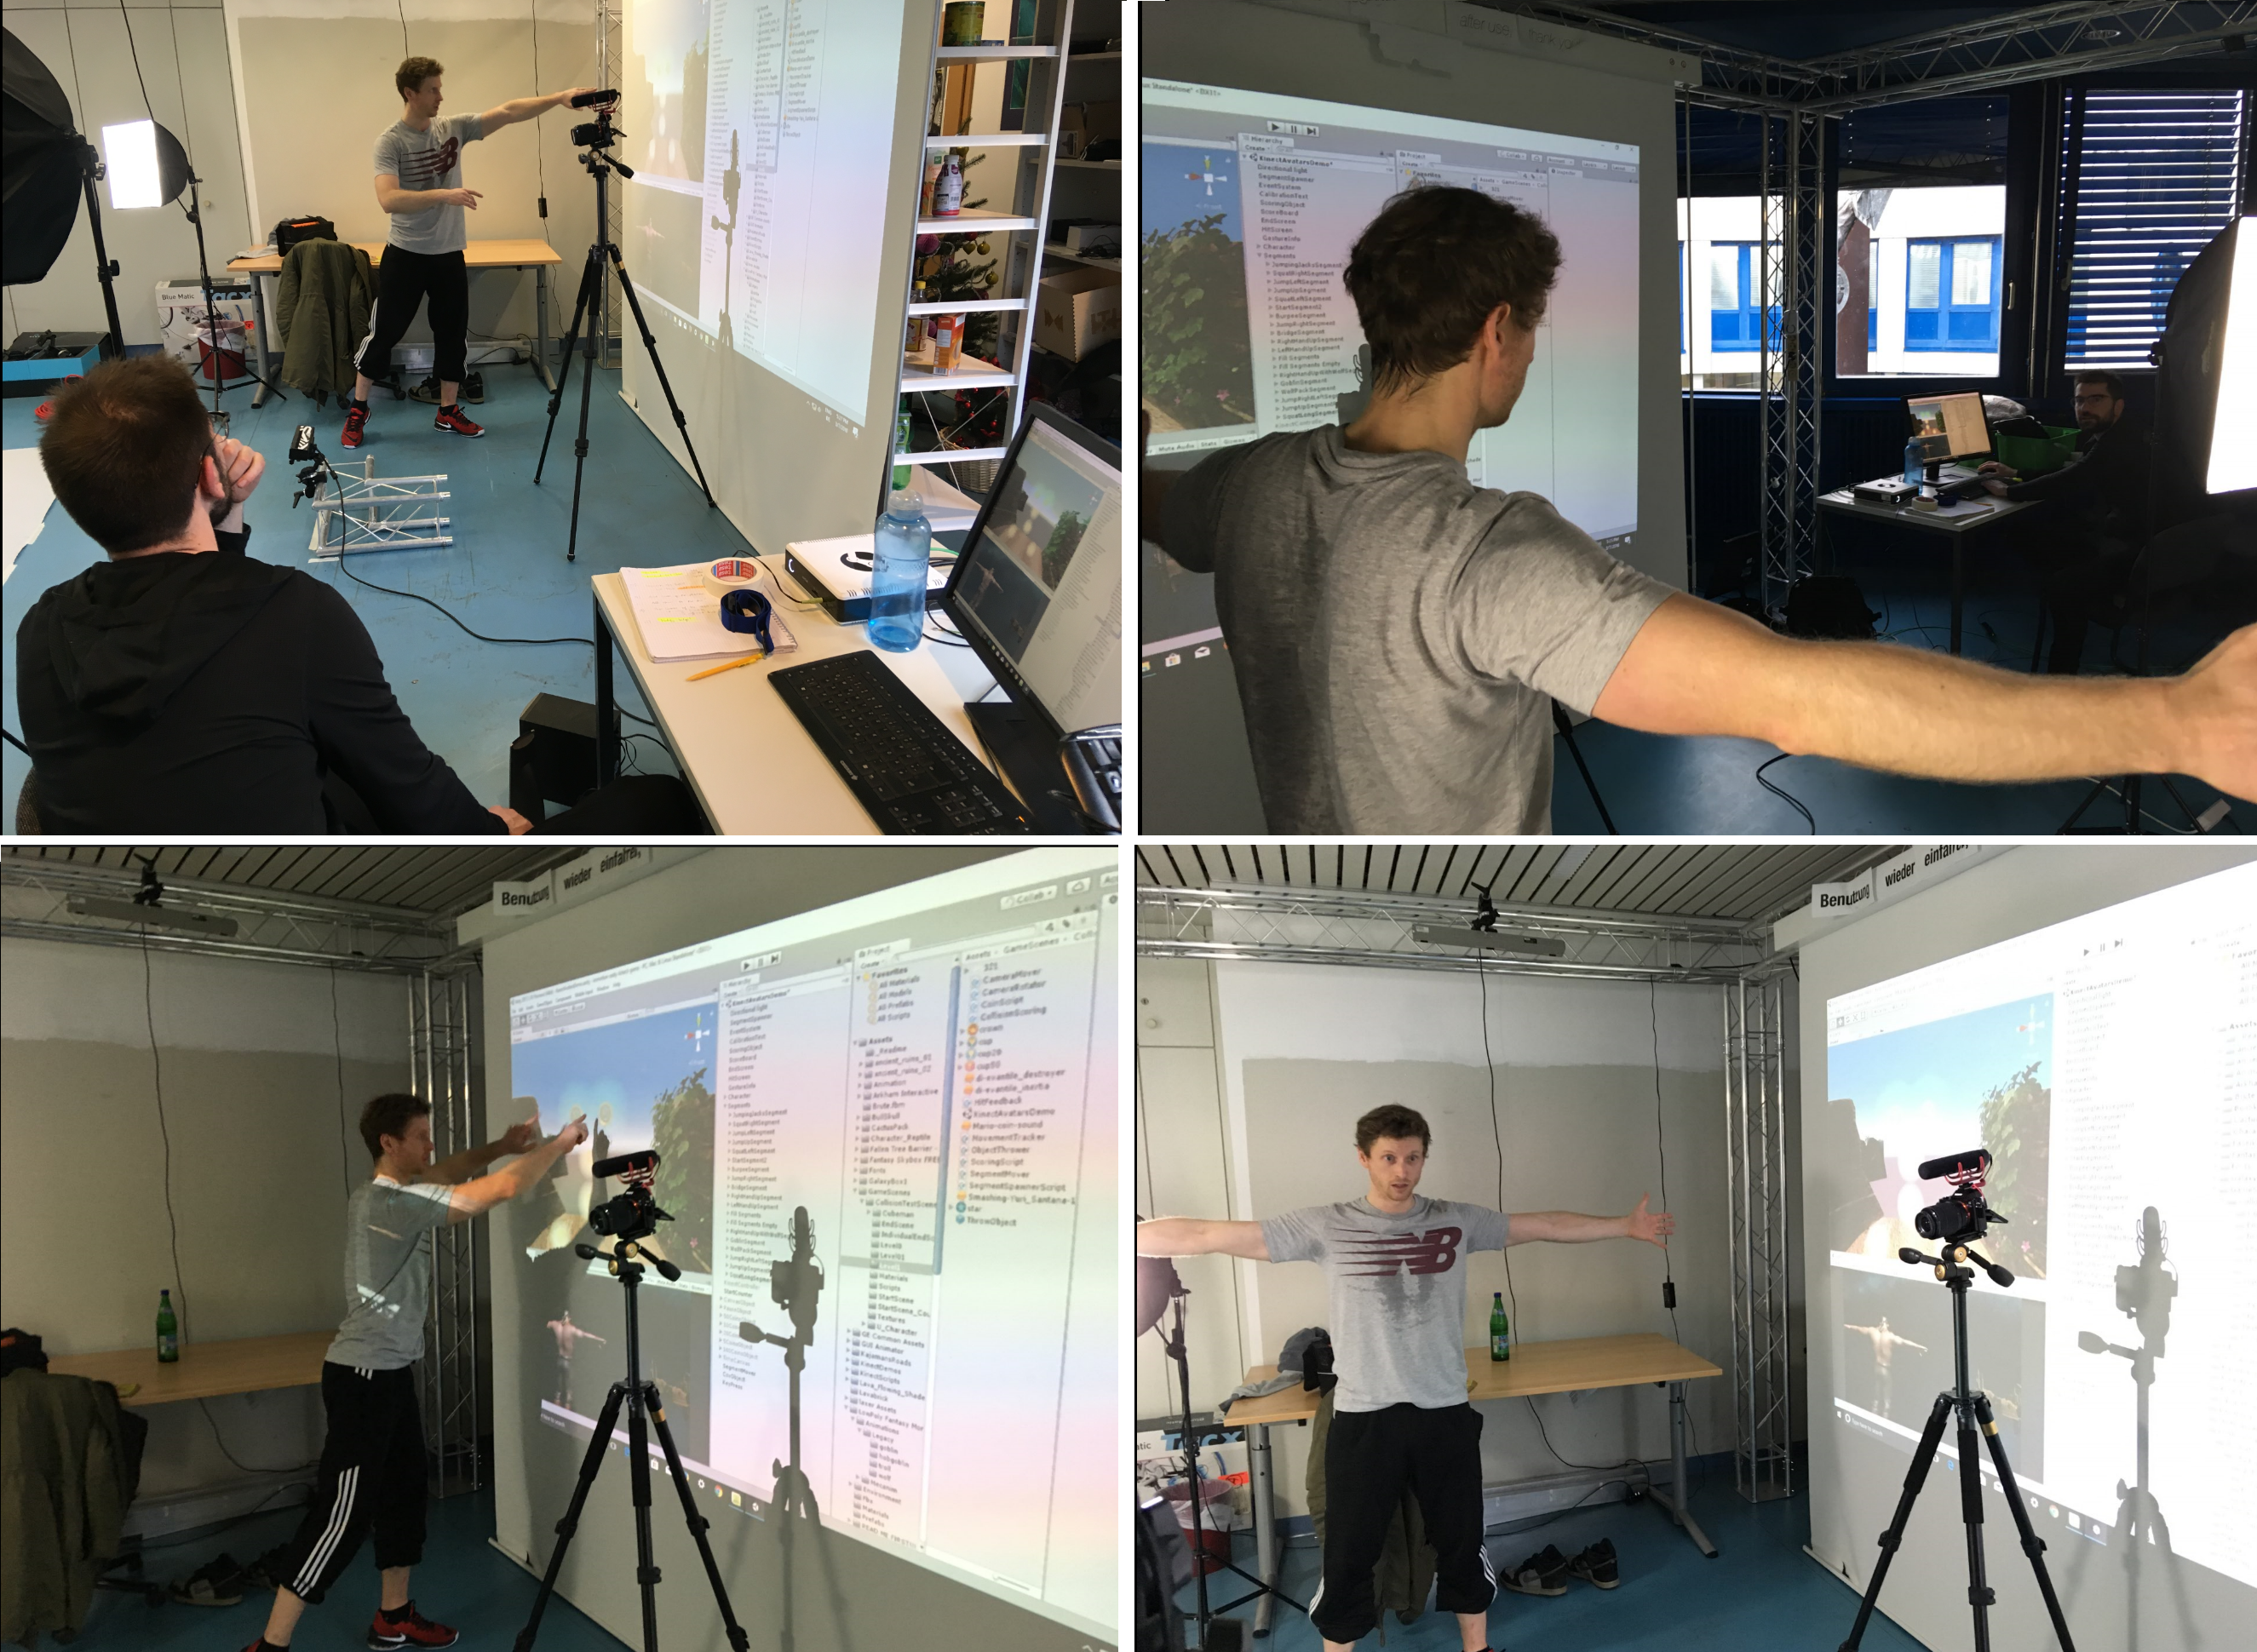
\includegraphics[width=\textwidth]{expertsDesign}
    \caption{Exergame related design discussions with fitness expert.}
    \label{fig:expDesign}
\end{figure}\\
In the next sections we describe and present the segments created as well as the movements that were required to be performed within them.\pagebreak
\section{Home Window Overview}
When the user starts the exergame, the \textit{Home screen} that is depicted in Figure \ref{fig:start} is showed. Apart from starting the game, other options are available for the user as well:
\begin{itemize}
\item Start
\item Help
\item Volume
\item High Score
\item Quit
\end{itemize}
\begin{figure}[h]
    \centering
    \includegraphics[width=\textwidth]{Start}
    \caption{Home screen.}
    \label{fig:start}
\end{figure}
Each of the above presented option opens a new window and provides the user with certain functions. Next, the above listed options will be further detailed.\pagebreak
\paragraph{Start Menu}
By selecting the \textit{Start} button in the Home screen, the user is presented with a new screen as showed in Figure \ref{fig:userinfo}. In this step, the user needs to input a username that will be used throughout the gameplay. The username does not have to be unique. In case it already exists, at the end of the game, all the scores achieved in previous game runs with the same username will be presented in ascending order by game scores as presented in Figure \ref{fig:individualScore}. By selecting \textit{Start} the exergame begins. By selecting \textit{Back}, the user is directed back to the Home screen.\\
\begin{figure}[h]
    \centering
    \includegraphics[width=\textwidth]{EnterName}
    \caption{User Info Menu.}
    \label{fig:userinfo}
\end{figure}
\paragraph{Help Menu}
The Help menu, as presented in Figure \ref{fig:help} lets the user know how to interact with the game, change the speed of the game, and start or stop the game. It also contains contact information for error reporting and user feedback. The Back button allows the user to go back to the Home screen.
\begin{figure}[h]
    \centering
    \includegraphics[width=\textwidth]{Help}
    \caption{Help menu.}
    \label{fig:help}
\end{figure}
\paragraph{Volume Menu}
The volume menu showed in Figure \ref{fig:volume}, gives users the possibility to modify the volume of the exergame's background music and sound effects (coins and obstacle collision sounds).\\
\begin{figure}[h]
    \centering
    \includegraphics[width=\textwidth]{Volume}
    \caption{Adjust volume menu.}
    \label{fig:volume}
\end{figure}
\paragraph{High Score Menu}
The high score menu depicted in Figure \ref{fig:highscore} ranks the users who played the exergame based on the points collected during one gameplay. The leaderboard displays the user's rank, name, score, and duration. This is a global leaderboard and it is different than the one presented in Figure \ref{fig:individualScore} since it includes all the users previously interacted with the game, their scores, and duration they played the game. Contrarily, the individual score board, displayed only at the end of each gameplay, shows the score and game duration of the user who currently interacted with the exergame. The Back button allows the user to go back to the Home screen.
\begin{figure}[h]
    \centering
    \includegraphics[width=\textwidth]{HighScore}
    \caption{High score menu.}
    \label{fig:highscore}
\end{figure}
\paragraph{Quit Menu}
The quit menu button was used for ending (closing) the game. 
\section{Game Start Overview}
For the purpose of tracking progress and achievements over time, users are required to input a name or username they would like to use during the gameplay. Based on the username, we display user's current score and position on the leaderboard during the gameplay and the highest scores at the end of the gameplay. The live score board and the leaderboard are presented  in Figure \textit{Individual score board} and Figure \ref{fig:individualScore}. After the user set the username and pressed the Start button, a \textit{Countdown window} as showed in Figure \ref{fig:counter} is presented to the user. The duration of the countdown is set to 5 seconds. We opted for this duration because it showed as the most optimal in our pilot study previously conducted with the university personal. This amount of time was sufficient for the users to prepare for the upcoming exercise by moving to the correct position. In case the user was not in the Kinect sensor range at the beginning of the game, a popup information window was displayed as showed in \ref{fig:waiting}. This information window was also displayed in case the connection to the Kinect sensor failed during the gameplay. \\
\begin{figure}[h]
    \centering
    \includegraphics[width=\textwidth]{Counter}
    \caption{Countdown window.}
    \label{fig:counter}
\end{figure}\\
\begin{figure}[h]
    \centering
    \includegraphics[width=0.6\textwidth]{LiveScore}
    \caption{``Live score'' during gameplay displayed in the left corner.}
    \label{fig:livescore}
\end{figure}\\
\begin{figure}[h]
    \centering
    \includegraphics[width=\textwidth]{WaitingForUser}
    \caption{``Waiting for user'' popup window.}
    \label{fig:waiting}
\end{figure}\\
Next, an overview of the game segments and corresponding movements required to perform in each of them will be presented.
\section{Game Segments Overview}
As already pointed out, each warm up movement the user was required to perform has been represented by a game segment. Following recommendations from experts, available literature, and the previously conducted online study, the list of warm up movements the users were required to perform during the game was updated. Additionally, we introduced so called \textit{filler} or \textit{empty} segments. In these segments no movements were required to be performed. They were placed between regular segments where movements needed to be performed. Their only purpose was to give users a short amount of time to prepare for the subsequent game segment. By generating all the segments randomly during gameplay, each resulting game map and warm up session induced by the map were unique. Moreover, our intention was to make the exergame intuitive to use. That is, the movements should come naturally to the users and should not require additional explanation. This was the result of our iterative and user centered design approach. We designed the segments based on the movements that can help users to warm up, and not contrarily. That way, every movement induced by obstacles and coins was executed correctly and came naturally to the player without additional explanation. Figure \ref{fig:topview} gives an overview of all the segments used in the exergame.\pagebreak
\begin{figure}[h]
    \centering
    \includegraphics[width=\textwidth]{SegmentsTopView}
    \caption{Overview of game segments - top view.}
    \label{fig:topview}
\end{figure}\\
In most of the segments depicted in Figure \ref{fig:topview}, one specific movement was required to be performed. Some segments were without obstacles and were present in order for the users to prepare for the next segment (and movements). Also, segments without any obstacles were used at the beginning of the exergame. At the very beginning of the exergame, ten filler segments were generated, however this number has been made adjustable. The empty segments were placed at the beginning in order to avoid any sudden movements by the player risking injuries. Moreover, not having to perform any movements gave the player time to adjust to the gameplay and prepare for the movements.\\
All the segments were designed to induce one of the following movement:
\begin{itemize}
\item Left hand up
\item Right hand up
\item Squat (short and long)
\item Jump
\item Star jump
\item Left hand down to the floor
\item Right hand down to the floor
\end{itemize}
Figure \ref{fig:rightup} shows the segment in which the user is required to move the right hand in the upper position and, in the same time, avoid the obstacle. In case the user comes in contact with the obstacle, one point is substracted from the overall user's score.\\
\begin{figure}[h]
    \centering
    \includegraphics[width=0.85\textwidth]{RightHandUp}
    \caption{Right hand up segment.}
    \label{fig:rightup}
\end{figure}
\begin{figure}[h]
    \centering
    \includegraphics[width=0.85\textwidth]{ExpertRightHandUp}
    \caption{Expert right hand up movement.}
    \label{fig:rightHandUp}
\end{figure}\\\\
Figure \ref{fig:leftup} depict the segment in which the user is required to move the left hand in the upper position in order to collect the coins. The obstacle was placed below the coins and one point is reduced from the user's overall score in case it was hit.\\
\begin{figure}[h]
    \centering
    \includegraphics[width=0.85\textwidth]{LeftHandUp}
    \caption{Left hand up segment.}
    \label{fig:leftup}
\end{figure}
\begin{figure}[h]
    \centering
    \includegraphics[width=0.85\textwidth]{ExpertLeftHandUp}
    \caption{Expert left hand up movement.}
    \label{fig:leftHandUp}
\end{figure}\\
In segments presented in Figure \ref{fig:wolfRight},  \ref{fig:goblin}, and \ref{fig:goblin} similar hand movements were required to be performed. The only difference was that in these segments the user is given a choice whether to go left or right. For instance, in Figure \ref{fig:goblin} player could collect four coins by moving to the right side. On the other hand, the user player could also go left and try to collect a blue coin that was worth five points. However, there was a possibility to lose points if collided with the obstacle.\\
\begin{figure}[h]
    \centering
    \includegraphics[width=0.85\textwidth]{HandUpRightWolf}
    \caption{Right hand up segment.}
    \label{fig:wolfRight}
\end{figure}
\begin{figure}[h]
    \centering
    \includegraphics[width=0.85\textwidth]{GoblinHandLeftOrRight}
    \caption{Right or Left hand up segment.}
    \label{fig:goblin}
\end{figure}\\\\
Figures \ref{fig:2wolfs} and \ref{fig:2sides} represent a segment where the player was also given an option to chose which movement to perform. Both the movements included rising hand in the upper position. The decision was left to the user. In case the user opted for the left side, the possible reward were two blue coins that were worth ten points in total. In case the user opted for the right side, the possible reward were three red coins that were worth nine points in total. However, there was a possibility to lose points by colliding with the obstacle.\\
\begin{figure}[h]
    \centering
    \includegraphics[width=0.85\textwidth]{2WolfsRight}
    \caption{Right or Left hand up segment.}
    \label{fig:2wolfs}
\end{figure}\\
\begin{figure}[h]
    \centering
    \includegraphics[width=0.85\textwidth]{TwoSides}
    \caption{Right or Left hand up segment.}
    \label{fig:2sides}
\end{figure}\\\\
In Figure \ref{fig:jumpleft} the user was required move to the left and touch the floor with the left hand in order to collect the coins. Moreover, the player was required to stay in that position for a short amount of time in order to collect all the coins.\\
\begin{figure}[h]
    \centering
    \includegraphics[width=0.85\textwidth]{JumpRight}
    \caption{Move left segment.}
    \label{fig:jumpleft}
\end{figure}
\begin{figure}[h]
    \centering
    \includegraphics[width=0.85\textwidth]{ExpertHandDownLeft}
    \caption{Expert left hand down movement.}
    \label{fig:expertLeftDown}
\end{figure}\\
In Figure \ref{fig:jumpright} the user was required move to the right and touch the floor with the right hand in order to collect the coins. As in previous segments, in case an obstacle was hit, the overall score was reduced by one.\\
\begin{figure}[h]
    \centering
    \includegraphics[width=0.85\textwidth]{JumpLeft}
    \caption{Move right segment.}
    \label{fig:jumpright}
\end{figure}
\begin{figure}[h]
    \centering
    \includegraphics[width=0.85\textwidth]{ExpertHandDownRight}
    \caption{Expert right hand down movement.}
    \label{fig:expertLeftDown}
\end{figure}\\\\
In in the segment presented in \ref{fig:rightleft} the player needed to move right and left. Compared to the similar movements depicted in previous figures, the movements in this segment needed to be performed much faster in order to collect the coins.\\ 
\begin{figure}[h]
    \centering
    \includegraphics[width=0.85\textwidth]{RightLeft}
    \caption{Move right and left segment.}
    \label{fig:rightleft}
\end{figure}
\begin{figure}[h]
    \centering
    \includegraphics[width=0.85\textwidth]{ExpertLeftRight}
    \caption{Expert right and left movement.}
    \label{fig:expertLeftRight}
\end{figure}\\
Figure \ref{fig:squatleft} and \ref{fig:squatright} show game segments where the user was required to perform similar movements as depicted in the previous figures. The main difference was that after moving right or left, additional squat needed to be performed in order to avoid the obstacle and collect the coins. In case the user hit one of the obstacle, the overall user score was reduced by one.\\
\begin{figure}[h]
    \centering
    \includegraphics[width=0.9\textwidth]{SquatLeft}
    \caption{Move left segment.}
    \label{fig:squatleft}
\end{figure}
\begin{figure}[h]
    \centering
    \includegraphics[width=0.9\textwidth]{SquatRight}
    \caption{Move right segment.}
    \label{fig:squatright}
\end{figure}\\
In Figures \ref{fig:jumpup} and \ref{fig:jumpssmallrock}, the user was required to perform a jump in order to avoid the obstacle and collect the coins. The obstacle depicted  in \ref{fig:jumpup} was the lowest in the middle. The user is presented with a choice of collecting a additional bluer coins if hands were also included in the movement. These blue coins were placed in a position that required higher jump and placing both hand in the upper position in order to be collected.\\
\begin{figure}[h]
    \centering
    \includegraphics[width=0.9\textwidth]{JumpUp}
    \caption{Jump up segment.}
    \label{fig:jumpup}
\end{figure}\\
Compared to the previous movement, the one needed to be executed in Figure \ref{fig:jumpssmallrock} did not require additional hand movement.\\
\begin{figure}[h]
    \centering
    \includegraphics[width=0.9\textwidth]{JumpSmallRock}
    \caption{Jump up segment.}
    \label{fig:jumpssmallrock}
\end{figure}\\
Figure \ref{fig:star} depicts a game segment where the user was required to perform a \textit{star} jump in order to collect all the coins.\\
\begin{figure}[h]
    \centering
    \includegraphics[width=0.85\textwidth]{JumpinJack}
    \caption{Star jump segment.}
    \label{fig:star}
\end{figure}
\begin{figure}[h]
    \centering
    \includegraphics[width=0.85\textwidth]{ExpertJump}
    \caption{Expert Star jump movement.}
    \label{fig:expertstarjump}
\end{figure}\\\\\\\\
Figures \ref{fig:squat} and \ref{fig:squatlong} depict game segments in which the user was required to perform a squat and by doing that collect coins. In case the user hit the obstacles placed above the coins, the overall score was reduced by one.\\
\begin{figure}[h]
    \centering
    \includegraphics[width=0.85\textwidth]{Squat}
    \caption{Squat segment.}
    \label{fig:squat}
\end{figure}
\begin{figure}[h]
    \centering
    \includegraphics[width=0.85\textwidth]{SquatLong}
    \caption{Squat long segment.}
    \label{fig:squatlong}
\end{figure}\\
\begin{figure}[h]
    \centering
    \includegraphics[width=0.85\textwidth]{ExpertSquat}
    \caption{Expert squat movement.}
    \label{fig:squatlong}
\end{figure}\\
Figure \ref{fig:bridge} is one of the filler segments used for the users to prepare for the next movement. However, in case the user does not use the bridge and comes in contact with the walls or lava obstacles, the user is looses a point.
\begin{figure}[h]
    \centering
    \includegraphics[width=0.85\textwidth]{Bridge}
    \caption{Bridge segment.}
    \label{fig:bridge}
\end{figure}\\
Figure \ref{fig:filler} depicts the filler (empty) segments that are placed at the beginning of the game and in between segments with obstacles in order to give players enough time to prepare for the subsequent movement.
\begin{figure}[h]
    \centering
    \includegraphics[width=\textwidth]{Filler1}
    \caption{Filler segments.}
    \label{fig:filler}
\end{figure}\\
Next, screenshots from game end will be presented and discussed in details.\pagebreak
\section{Game End Overview}
The player ends the game when she feels warmed up enough for the subsequent physical activity. When the game ends, the player is displayed the \textit{Individual score board} that is showed in Figure \ref{fig:individualend}.\\
\begin{figure}[h]
    \centering
    \includegraphics[width=\textwidth]{IndividualEndScene}
    \caption{Individual end scene.}
    \label{fig:individualend}
\end{figure}\\
Based on the player's username we display all the previous scores. The scores are displayed in descending order by the points achieved during each game run. The player is also presented with the duration each game lasted and the personal best score. By selecting the \textit{Back to main menu} button, the player can go back to the Home screen. 

\label{endgamelabel}

%\chapter{Study Design}\label{chapter:studydesign}

\section{Description of the Experiment}

In order to critically evaluate our system, after the features of our prototype exergame are evaluated in the first stage and the second version implemented, we pilot-test and assess it through a second survey. In the this stage, we test the motivational and guidance features of our system. For this purpose a between subject experiment is conducted with 20 participants. 

\subsection{Introduction and Goals} 
Introduce your experiment, and give the reader the specific goals you expect it to address. It is common at this stage to give the reader a hint of your hypotheses (if they are not already hinted at in the Introduction).
\subsection{Methods} 
In order to address the research questions outlined in XX, we implement and test an exergame for warm up exercises before sports activities. 
%This is a detailed description of the experiment that should allow other researchers (familiar with HCI and experimental design in general, but not familiar with your experiment) to replicate your experiment.%
\subsubsection{Participants}
Describe your participants (e.g., any relevant demographics, if/how they were divided into categories), including total number, and recruiting approach. Indicate if any incentives were used. Comment on the representativeness of your participants relative to the target population, if their representativeness isn’t immediately obvious.
\subsubsection{Conditions}
If your experiment is comparing multiple different interfaces or interactive systems or techniques, describe each of them. Screen snapshots of interfaces/systems are particularly useful.
\subsubsection{Tasks}
Briefly describe what participants were asked to do with the interactive system(s).

\subsubsection{Design}
Write the formal experimental design (e.g., a 2 x 3 mixed factorial design, more specifically a 2 levels of expertise (between subjects) x 3 interfaces (within subjects) design).
\subsubsection{Procedure}
%Describe the sequence of activities each participant followed. This should document the experiment from a participant’s perspective, from the moment s/he arrives (e.g., a preliminary questionnaire to obtain X information, followed by five tasks with system A, then a 10 min break, followed by the same five tasks with system B, and finally a semi-structured interview to solicit opinion on Y).%
The activities each participant of the experiment session followed is presented in this section.\\ 

Before the experiment, the lab environment is set up. The Kinect sensor is placed in a correct position, the projector is turned on. In each session only one participant is present and guided by the researcher. The activities each participant >>> are as follows:
\begin{itemize}
\item The researcher explains the sensors and tools that are required for the experiment, after which the participant puts them on. The sensors used in each session include a heart rate monitor and Microsoft Band. In order to measure the range of motion around a joint in the body, a goniometer is utilized. %maybe kinect could do it%
After the researcher confirms that the sensors are placed in a correct position, we start recording heart rate data and WHATEVER WE DO WITH THE BAND.
\item For each participants we measure ROM of the following joints using double-armed goniometer. %ovo mozda na pocetku%
\item After the measurements are completed, the participant rests for up to 10 minutes in order to take the readings of the resting heart rate. 
\item While the participant rests, the researcher explains and presents the movements that are required from the participant to perform during the experiment. Furthermore, the researcher explains how the game is played.
\item When the rest period completes, the participant is asked to practice the required movements.
\item In order to avoid starting the game and warm up with already stimulated heart rate, the participant is required to rest for 5 minutes. 

\item The participant is asked to prepare for the warm up by positioning to the position marked by the researcher. 
\begin{itemize}
\item  If this participant is part of the experimental group, the game starts with the start scene where the participant enters his or her name. After 5 seconds, the game proceeds with scenes in which the participant performs the previously presented movements in order to avoid obstacles and collect coins. The duration of the game is not fixed and it is played up to the point when the participant feels warmed up enough. During the experiment, the warm up procedure performed by the participant is recorded. %this reformulate%

\item  If this participant is part of the control group, the video that shows a gameplay performed by another participant who was part of the experiment group. The participants performs the same movement as in the playing video. As with with the sessions in the experiment groups, the duration of the warm up is not fixed and the 
video is played up to the point when the participant feels warmed up enough. During the experiment, the warm up procedure performed by the participant is recorded.
\end{itemize}
\item After the participant finished with the warm up, he or she takes a rest. During this period the researcher assesses the ROM of the participant. 
\item The participant in the experiment group plays the game and the participant in the control group watches the video for the second time with the same content as previously. This results in more heart rate data, and allows more opportunity for the player
to experience psychological flow, as discussed in section 3.6.1. Another 10 minutes of play time
brings the total exposure to about 20 minutes plus the break. OVO MODIFY
\item With the game complete, the participant removes the sensors, rests and completes the survey. MODIFY
\end{itemize}
\subsubsection{Apparatus}
Describe the physical setup of the experiment (e.g., where was it conducted, on what kind of equipment, etc.)
\subsubsection{Independent and Dependent Variables}
Include exactly how you intend to measure each dependent variable. 
\subsubsection{Hypotheses}
Remember to state these in terms of the independent and dependent variables. If it is not immediately clear why you would have a certain hypothesis (it often follows logically from the introduction of the experiment), then include a brief explanation separate from but following the hypothesis. You do not need to state the null hypothesis.
\subsection{Problems/Limitations}
Describe any problems/limitations encountered that will help other researchers avoid or account for them if they decide to replicate your experiment.
\section{Results}

This section is an objective report on what the numbers show. You should not try to interpret the meaning of the numbers in this section. Some of the things you may do here are: 
report means and standard deviations in neat tables 
indicate the statistics used and levels of significance 
include graphs, plots, histograms, etc that tell a story about the actual figures obtained 
Only critical raw data and summary statistics should be included in the actual report. However, you must keep all your raw data in a separate archival report, should anyone (a reviewer in the case of real scientific reporting) need more detail than is provided in the paper. 
\section{Discussion}
Interpret the results. Although you should still try to be as objective as possible, the discussion section should illuminate your critical thinking about the results. Explain what the statistics mean, account for anomalies, and so on.
\subsection{Interpretation of Results}
Discuss what you believe the results really mean. For example, if you find a significant difference for some effect, what does that mean to the hypothesis? Is the different seen an important one?
\subsection{Relation to other works}
How do the results you’ve obtained relate to other research findings?
\subsection{Impact for practitioners}
As computer scientists, we are particularly concerned with the implications of our findings on practitioners. Should existing interface constructs be designed differently or used in a new context? Do you have suggestions for new designs? How can the findings be generalized?
\subsection{Critical reflection}
Critical reflection is one of the key foundations of science. You should criticize your work (constructively, if possible), indicate possible flaws, mitigating circumstances, the limits to generalization, conditions under which you would expect your findings to be reversed, and so on.
\subsection{Research agenda}
The best experiments suggest new avenues of exploration. In this section, you should reflect and refine your hypotheses, describe new hypotheses, and suggest future research, ie research that you would do if you continued along this path.
\section{Conclusions}
Summarize the report, and speculate on what is to come.
Acknowledgements. This section should give thanks to the major people (supervisors, associates) and organizations (sponsoring agencies, funders) that helped you. For example, I would like to thank Ben Shneiderman, whose report framework was used to build this one.
%\chapter{Conclusion}
\label{chap:conclusion}
In this paper we presented a development and evaluation process of an exergame for warm up guidance and motivation that is specifically targeted towards amateur athletes who rarely or never warm up before physically strenuous exercises and sports activities. We used Kinect sensor in order to track and capture players' movements and dispayed the exergame on the wall using a projector. By placing various game obstacle and coins in a specific position, our intention was to indirectly promote exercise through the gameplay of repeatedly performing warm up related movements chosen after related literature review and discussions with fitness experts.\\\\The development of our exergame consisted of three phases that included requirements gathering, prototype development with user evaluation, and final exergame development with further user evaluation. The first phase was an exploratory step in which we justified the development and identified currently available commercial and non-commercial solutions. In our research, we did not find any available solution with primary focus on warm up as a preparatory activity. In the second phase we implemented and evaluated our exergame prototype. The prototype was a scaled down version of our final exergame solution.  In order to evaluate our prototype, we created an online survey. The purpose of the survey was to explore general work out and warm up habits of the respondents, as well as their preferences and general acceptance of gamified solutions of warm up exercises.  Total number of n = 446 individuals participated in the online survey. With respect to respondents' warm up preferences before a physical activity, n = 251 (56.3\%) reported always warming up, whereas n = 195 (43.7\%) reported not warming up regularly before physically more demanding exercises. The results regading the reasons for avoiding warm up exercises aligned with the ones presented in \cite{fradkin2010effects}. This further justified the need for educational and motivational solutions, which are enjoyable and easy to carry out, with primary focus on the major muscle groups and benefits of warm up, in order to increase the proportion of athletes who engage in warm up routines before every exercise. The prototype exergame and one short warm up session has also been presented in the online survey. \\Total of n = 269 (60.31\%) respondents reported that would use the prototype exergame for warming up. Out of n = 195 respondents who reported not warming up before sports activities n = 124 (63.58\%) stated that they would use the presented solution as a tool for warming up before sports activities. Based on the results obtained from the survey, comments, and suggestions, in the third phase the prototype version of the exergame has been redesigned in order to better suit the needs of its future users. We opted for a modular design, consisting of multiple game segments each containing different obstacles that induced different movement during gameplay. These segments were generated procedurally on random and were easily modifiable. Our primary goal in the last phase was to investigate if our solution can be used to guide athletes through the warm up process efficiently. Despite some limitations, our exergame showed higher results and statistically significant difference in terms of exercise duration, physical activity enjoyment, and perceived exertion level compared to the non-gaming session under the same conditions. The exercise movements that were required to be executed during gameplay felt intuitive and came naturally to the participants. Thus, we concluded that the exergame provided adequate guidance in performing a general warm up procedure. Contrarily to expected results, the evaluation of psychological and emotional dimensions  did not show significant differences between two conditions. These results were most likely due to the fact that both conditions involved the usage of immersive technology and a novel approach (game with Kinect sensor and a warm up video) that succeeded in shifting the participants' focus from the discomfort and dullness of the exercise, but the results showed that the exergame condition offered a more immersive and enjoyable experience.\\\\
Based on the results obtained in this paper, we conclude that exergames with incorporated immersive technologies can be used  as a guiding tool for general warm up procedures and can offer significant benefits as motivational tools to promote engagement in warm up exercises for amateur athletes. Moreover, the exergame design given in this paper was shown to be effective in promoting the desired health outcomes in terms of increased range of motion and expected heart rate recommended by previous studies and medical experts.  Lastly, the modular design approach that have been followed in the development of the final version of our exergame solution has been effective for game segment customizations and adjustments. This, further, makes the game easily extensible in case additional movements need to be incorporated for future use cases. Future studies investigating exergames should consider the design approach introduced in this paper, such as the modular design of the game segments, the procedural generation of the exergame environment, and the advantages of immersive technologies.\pagebreak
\section{Future Work}
This paper has tackled several interesting areas worth considering in future works. 
Firstly, our solution has been designed for general warm up exercises in mind. This means that the movements induced in various game segments could be executed without any prior knowledge of the exercise. However, based on the surveys conducted and the results collected, the respondents who declared themselves as professional athletes found the required movements too general and not applicable for the sports they engage in. Hence, generating versions of the exergame that are designed for certain sports areas, and require previous knowledge of the movements might be worth considering. This way, our solution could be used not only in gyms by amateur athletes, but have more diverse players pool. Secondly, due to hardware constraints, our solution did not take into account the correctness of the movements executed. As pointed out, we opted for general movements that are intuitive and easily executed. Interestingly, we observed that some of the players struggled at the beginning of the gameplay to execute the movements correctly. This resulted in two scenarios. Either the player missed collecting the coin and hit the obstacle, or the coin was collected but the movement was faulty. It would be interesting to see how effective our solution would be in not only guiding the players through a warm up procedure, but in the same time, correcting the movements that are not executed properly. Lastly, survey respondents and study participants indicated an interest of having a possibility for a collaboration during gameplay in a form of a group warm up or a competition. Previous studies already showed that introducing competition in a form of scoreboards can be a powerful motivator for certain player types \cite{ werbach2012win, zichermann2011gamification}. Having this in mind, our solution also incorporated game elements suitable for more competitive player types and assessed their effects and acceptance. Even though our exergame in it's current design is not well suited for collaborative warm up session that include multiple players at the same time, the existing high score system could be extended in a way the results are shared on social media platforms further enhancing the competitive aspect. Alternatively, the exergame could be extended in a way it allows multiple players to perform a warm up procedure in the same time, either collaborating or competing among each other. 
%\chapter{Appendix}\label{chapter:appendix}
\includepdf[pages=-]{myfile.pdf}
\includepdf[pages=-]{myfile.pdf}
\includepdf[pages=-]{myfile.pdf}
\includepdf[pages=-]{myfile.pdf}
\includepdf[pages=-]{myfile.pdf}

%\input{appendices/injury_causes}


% *************** Bibliography ***************
\bibliographystyle{ieeetr}
{\small\bibliography{bibliography/reference}}
\clearpage

% *************** Appendixes ***************
\addtocontents{toc}{\vspace{2em}}
%\appendix
\appendixpage
\includepdf[pages=-, offset=75 -75]{AdditionalDocument/ReviewBoard_Response.pdf}
\includepdf[pages=-, offset=75 -75]{AdditionalDocument/studyPoster_ver2.pdf}
\includepdf[pages=-, offset=75 -75]{AdditionalDocument/studyPoster.pdf}
\includepdf[pages=-, offset=75 -75]{AdditionalDocument/PRE-STUDY-DemographicSurvey.pdf}
\includepdf[pages=1, offset=75 -75]{AdditionalDocument/parQandSafety.pdf}
\includepdf[pages=-, offset=75 -75]{AdditionalDocument/BSA-F.pdf}
\includepdf[pages=-, offset=75 -75]{AdditionalDocument/PACES.pdf}
\includepdf[pages=-, offset=75 -75]{AdditionalDocument/STUDY-1-BorgRPE_Scale.pdf}
\includepdf[pages=-, offset=75 -75]{AdditionalDocument/SUS.pdf}
\includepdf[pages=-, offset=75 -75]{AdditionalDocument/Post-study-Exp.pdf}
\includepdf[pages=-, offset=75 -75]{AdditionalDocument/Post-study-Control.pdf}
Post-study-Exp
% *************** Back matter ***************
%\backmatter
%\input{back.tex}
\end{document} 
